\documentclass[12pt]{article}
\usepackage[english]{babel}
\usepackage[pdftex]{graphicx}
\usepackage[latin1]{inputenc}
\usepackage{verbatim}
\usepackage{listings}
\usepackage{amsfonts}
\usepackage{color}
\usepackage{epsfig}
\usepackage{fancyvrb}
\usepackage{listings}
\usepackage[colorlinks=true, linkcolor = black, urlcolor  = black, citecolor = black, filecolor = black ]{hyperref}
\usepackage{subfigure}
\date{}

\setcounter{secnumdepth}{4}%
\setcounter{tocdepth}{4}% 

\lstset{
  %backgroundcolor=\color{gray},
  frameround=fttt,
  stringstyle=\ttfamily,
  language=python,
  basicstyle=\small
}

\newcommand{\bigtilde}{$\sim$}
\definecolor{unih}{RGB}{1, 178, 170}
%% \def\framework{\textsc{Report}}

%\advance\textwidth by -1truecm
%\advance\oddsidemargin by 1truecm
%\advance\baselineskip by \baselineskip

\begin{document}

\begin{titlepage}
%%   \pagecolor{unih}
  \begin{center}
%%    \textbf{\uppercase{University of HertfordShire}}\\
%%     \hbox to \textwidth{\hrulefill}    
    %\fbox{
    \uppercase{ \textsf{
        \LARGE{\framework{}} \\ 
        \vspace{0.5truecm}
        \large{an exocentric vision framework for mobile robot teleoperations}
    }}
    %}              
    \hbox to \textwidth{\hrulefill}
    \vfill
    \vspace{0.5truecm}
    \includegraphics[width=150pt]{img/unict_logo.png}  %logo
    \includegraphics[width=300pt]{img/camera_frustum}
    \vfill
    
    \begin{flushright}
      \textsf{Students:} \\
      \textsf{\textbf{Daniele Ferro}} \\                      
      \textsf{\textbf{Loris Fichera}}
      \vspace{0.5 truecm}
                
      \textsf{Supervisors:} \\
      \textsf{\textbf{Prof. Salvatore Livatino }}\\
      \textsf{\textbf{Prof. Giovanni Muscato }}\\
    \end{flushright}
    
    \vspace{0.5 truecm}
    %%    \begin{figure}
%%    \end{figure}
    
  \end{center}
  
\end{titlepage}

\setlength{\baselineskip}{1.3\baselineskip} %per 30 righe in ogni pag.

\newpage
  % Frontpage
%% \section{State of the art}
\label{stateart}
%

%
Display used for common Head Mounted Display (HMD) are 
various, we try to explain the chief differences. In the
following we will examine five types: LCD, AMLCD, LCOS, 
FLCOS, OLED.
%

%
\subsection{LCD}
The LCD technology is based on the light modulating properties 
of liquid crystals (LCs). Since LCs are not able to emit light 
directly, actual LCD panels and displays need a light source.
%
That is why such devices are often classified as "passive" 
displays. 
%
LCD displays are usually for a general purpose use, but they 
can also be tuned for a specific usage - e.g. the displaying 
of highly detailed still images or of highly dynamic, 
fast-changing video content.
%
Because of their versatility, they are used in a wide range 
of applications including computer monitors, TVs, aircraft 
cockpits. They're also common in electronic consumer devices 
such as video player, gaming devices, etc.
%
Compared to other display-making technologies - such as CRT - 
LCD allows to make wider and flatter displays while reducing 
electrical power consumption and, thus, making LCD displays 
also well-suitable for mobile devices.
%

%
\subsection{AMLCD}
Active Matrix LCDs (AMLCD) use a matrix of thin-film transistors 
(TFTs) to achieve better performance compared to normal LCD screens. 
They still have polarizing sheets and cells of liquid crystal 
(same as LCD), but the TFTs allow to store the electrical state 
of each pixel on the display while all the other pixels are 
being updated.
%
The advantages of a TFT-LCD monitor are many. It provides a 
larger viewing-angle and a much brighter display than a passive 
matrix monitor with the same size. Some designs have replaced 
transistors with other components such as diodes.
%
With an active matrix only the desired pixel receives a charge, 
acting as a capacitor and holding the charge until the next refresh 
cycle (transistors have the ability to hold a charge for a limited 
period of time). On the contrary, a passive matrix display delivers 
current to the liquid crystals in a specific area with a simple 
conductive grid. AMLCD can be more accurate because, thanks to 
the switching action of transistors, only a the specific pixels 
receive a charge, improving image quality with respect to a 
passive matrix display.
%
AMLCDs are most popular type of display on the market today.

\subsection{LCOS}
Liquid crystal on silicon (LCOS) is a {\it micro-projection} or 
{\it micro-display} technology typically applied in projection 
televisions. It is a reflective technology and uses liquid crystals.
%
LCoS displays are well-suited for high resolution and high contrast 
images. 
%
There are two broad categories of LCoS displays: three-panel and 
single-panel. In three-panel designs, there is one display chip 
per color, and the images are combined optically. Single-panel 
designs, instead, makes use of only one display chip  that shows 
the red, green, and blue components in succession with the 
observer's eyes relied upon to combine the color stream. 
%
If the frequency of the color fields is lower than about 540 Hz, 
an effect called "color breakup" is seen, where false colors 
are briefly perceived when either the image or the observer's 
eye is in motion.
%

%
\subsection{FLCOS}
FLCOS devices are made using ferroelectric liquid crystals 
(so the technology is named FLCoS), which are inherently faster 
than other types of liquid crystals.
%

%
\subsection{OLED}
The Organic Light Emitting Diode (OLED) takes advantage of an 
electroluminescent layer, made of organic compounds, used 
like a LED. This layer is wrapped between two electrodes and 
at least one of the electrodes is transparent.
%
OLEDs are a young display technology, not yet able to emit as 
much light per unit area as an inorganic solid-state based LED. 
For this reason OLED are not used as point-light sources.
%
This devices can be used for multiple applications, from 
television and computer screens to small and portable system 
screens such as mobile phones, PDAs and head-mounted displays 
(where high-resolution is needed).
%
Since OLED displays do not require a backlight, they can 
perform deep black levels and be thinner and lighter than 
LCD panels. Besides, OLED displays can achieve higher contrast 
ratios. Even the power drain is lower, compared to LCD screen.
%

%
\subsection{A comparison towards displays}
By using AMLCD display for Head Mounted Display (HMD) the entire 
device is more compact, because AMLCDs only need a flat backlit 
panel rather than a complex (and thicker) illumination unit. 
This is the reason why FLCOS and LCOS displays are commonly not used. 
%
On the other hand, AMLCD display has relatively low contrast ratio 
and provides the lowest luminance range and largest pixel dimensions 
among all of the previously seen technologies.
As well as AMLCD, OLED offer a compact system design due to its 
self-emission nature. In addition, OLEDs provide a good range of 
luminance, even tough the resolution and contrast ratio of 
existing OLEDs are relatively low compared with FLCOS and LCOS microdisplays.
%
Besides, OLEDs life span would be shortened if the display 
luminance is high (e.g. more than 100 cd/m2).
%
According to \cite{Zhang:08}, for HMD designs a display panel around 2.50 cm is 
preferable as it would offer a good balance of compactness and the 
focal length range of the optics. In fact, when dealing with small 
display panels, shorter focal length and larger magnification are 
required in order to achieve a reasonable field-of-view (FOV). 
%
LCOS microdisplays offer the highest resolution and contrast compared 
with other types of displays and they are commonly used as image 
sources in digital projectors. 
%

%
\begin{figure}[!h]
  \begin{center}
    \includegraphics[width=400pt]{img/hmd_comparison_table.jpg}  %logo
  \end{center}
\end{figure}
%

%
The liquid crystal used in LCOS microdisplays, however, has low 
switching speed, which makes it impossible to use color sequential 
method, to achieve a full color mode. FLCOS offers high pixel 
resolution, luminance output, image contrast, and optical efficiency. 
Also, the fast response speed of ferroelectric liquid crystal makes 
it possible to achieve full-color display using a single-panel color 
sequential scheme. On the other hand, it requires a carefully designed 
illumination unit to achieve high contrast and high luminance, which 
makes the overall display system less compact than a system using 
AMLCD or OLED microdisplays.

\section{The Exocentric vision issue}
\label{sec:exo}
\subsection{Why use exocentric vision?}
Teleoperated mobile robots prove to be extremely useful 
when there is the need for performing operations in places that 
are unaccessible or dangerous for human beings - e.g. 
search-and-rescue missions within unknown regions or into 
collapsed buildings, caves, etc.
%
The supervisors' research group has been widely involved 
during the last years in the research on teleoperated robots. 
[citation needed].

As for the testing platform, they have been using 3morduc,
a differential-drive mobile robot - showed in figure \ref{fig:morduc} -
equipped with a pair of Videre Design [citation needed] 
stereo cameras and a laser scanner.
They have been focused on the making of a reliable software 
infrastructure which makes able a remote operator to drive 
the 3morduc in a comfortable fashion.
%% parlare dei campi di ricerca coinvolti?
%
\begin{figure}[!h]
  \begin{center}
    \includegraphics[width=200pt]{img/3morduc}  %robot pic
    \caption{The 3morduc robotic platform}
    \label{fig:3morduc}
  \end{center}
\end{figure}
%
[Indeed],our work focused on the robot-operator interaction and, 
hence, on how to improve such interaction. Analyzing previous work 
and data produced by the supervisors' research group, it emerges 
that the stereo cameras mounted on top of 3morduc, were used to 
provide the remote operators a \textit{first-person} point of view. 
In literature, such a system is also called an \textit{egocentric} 
vision system.
%

%
According to \cite{sugimoto}, \textit{by observing the camera image 
without an efficient human interface system, the operator 
tends to misinterpret the robot's position and direction}. This is 
due to the fact that  \textit{it's difficult for an
operator not accustomed to the vehicle to estimate the
vehicle's position and direction and the distances to a
target strictly based on camera images from the firstperson 
viewpoint}.
%
In order to improve the interaction between the robot and the operator 
an exocentric camera would be effective since it would provide a 
representation of the robot in the operating environment and, thus, 
a better understanding of where the robot is located into the environment 
and its actual direction.
%
Unfortunately the use of an exocentric camera is not trivial: for example, 
it could be mounted on a [dedicated long support] on the back of the robot, 
but such a support would terribly disturb the robot activity and its 
moving abilities. [di fatto e` un vincolo in piu` che si sta aggiungendo]
%
Non solo, una immagine precedente, contiene informazioni ambientali piu' 
ampie rispetto a quelle di una camera montata sul posteriore del robot.
%
To avoid such complications, \cite{sugimoto} proposes 
\textit{Time Follower's}, an approach to provide a virtual exocentric 
view.
%
%
\subsection{Time Follower's: an overview}
Time Follower's aims at providing an exocentric view of a mobile 
robot using an egocentric-mounted camera. The approach is simple: it is 
based on the use of previously recorded first-person images to provide 
comprehensible third-person imagery. A 3D representation of the robot 
is overlapped to such images in order to get the work done.
%
Key issueof the system are:
\begin{itemize}
\item how to choose the \textit{best} image
\item how to determine the \textit{right} place to draw the robot
\end{itemize}
%
    [a brief description of the two concepts]
%


\section{Setting up a Morduc simulator}
\label{sec:simulator}
A basic exocentric vision system for Morduc would need, 
at least, some images captured from the camera mounted 
on top of it and, for each image, the actual position of 
the robot at the time it was captured.
%
While images could be used as a texture on which draw 
a 3d represenation of the robot, informations about 
position are essential in order to draw the robot 
consistently, i.e. in the position the observer would 
see it if he was seeing the robot by means of an actual 
external camera.
%

%
An exocentric vision systems performs at its best 
when there's a large static space where the robot can move in. Since 
the real robot can not be easily teleguided in wide 
environment because of its size and the lack of a large 
room in Catania, where the robot is situated, a simulator 
has been used to reproduce the best set of data. The 
simulator can be thought of as a server, which receives 
requests and returns responses: the first are the commands 
sent by the user to move the robot, the latter the 
egocentric images and the robot position data.
%

%
Furthermore, with a simulator is extremely easy to 
change the environment where the robot is teleguided, 
so we can test the exocentric vision with an infinite 
number of environments without physically moving the 
robot in different places. In this way software 
development of exocentric vision can be faster, because 
it is simple and immediate to establish several test cases.
%

%
The first simulator adopted was Rosen\cite{rosen}. Written in 
Erlang \cite{erlang}, Rosen has been developed at the University
of Catania in order to simulate the behavior of robot with 
features completely different from Morduc. The chief one 
was that the robot had its own algorithm to set its movement, 
it was indeed not guided by a human operator. 
%

%
Rosen was used a couple of years ago for robot taking part 
in Eurobot competition\cite{eurobot},
but for our purpose was not fit since it does not even 
provide a egocentric vision. The difficulties faced to edit 
Rosen made us to look for a more suitable simulator.
%

%
In 2006, at the Aalborg University, the Italian student Filippo 
Privitera wrote a simulator to teleguide the Morduc robot 
\cite{privitera}. The simulator reproduces the robot (drawing its 
physical features) situated in a room with a variable numbers 
of walls. Walls' position is specified by the user, by giving 
the simulator a black and white bitmap image with the room 
plane to build the whole environment from. 
%

%
Besides, Privitera's simulator allows to enable the 
stereoscopic vision, with anaglyph or polarized method (both 
types are applied on the egocentric camera). These features 
make not too tricky to implement the exocentric vision control 
with 3d effect, in order to improve the user's ability in 
moving the robot. Other information like the number of collisions 
or the robot distance from the nearest obstacle are provided 
by simulator.
%

%
This simulator was written in MFC (Microsoft Foundation Class) 
framework and has been used for testing user ability in
driving the robot, in comparison with the real robot server 
to quantify the differences between the two facilities. 
For more information see \cite{privitera}.
%

%
With a simulator specifically built for the Morduc robot, it 
was not difficult to edit the source code to obtain what we 
needed. First of all, we needed to record data about egocentric 
vision and robot status, because they are the input value 
of the exocentric vision simulator. In order to achieve this, 
we edited the source code to allows the user to store data: by 
pressing the 'P' key keyboard the actual information (e.g. the 
actual camera image and robot status) are recorded in log files.
%

%
Every session in Privitera's simulator has its own identifier 
(a integer number). When the 'P' key is pressed the simulator 
write a new line in the text file named 'data\_$\langle$number 
of session$\rangle$.txt', creating the file if it does not 
exist. Each line contains four float number values, with the 
following meaning:
%
\begin{enumerate}
\item x coordinate
\item y coordinate
\item theta value (in radiant s)
\item timestamp
\end{enumerate}
%
where the timestamp refers to the beginning of the simulation.
%

%
Beside the text file there are several PNG files, each for every 
line written in 'data\_$\langle$number of session$\rangle$.txt'. 
These files are named 'screenshot\_$\langle$number of 
session$\rangle$\_$\langle$timestamp$\rangle$.png', where the 
number of session indicates for every screenshot 
- i.e. the egocentric vision - the proper text file, and the 
timestamp the line with the associated status of the robot.
%

%
The software which implement the exocentric vision control 
will look for text and image files related to a specific 
session, in order to read the necessary input and draw the 
robot correctly. It must be able to choose the right image 
to use as background, among those previously read; to draw 
the robot over the background in the right position and 
orientation, depending on its route; to prevent or signal 
collisions to the user, and so on.
%

%
Future development can reach a more interactive collaboration 
between simulator and exocentric vision control program. For
example, it would be better if the control program could 
interact (by a socket or another data stream) with the 
simulator, sending the movement command and retrieving 
information about robot status. In this case log files 
would be substituted by a local or global connection, 
and the exocentric program would not read information from 
file (as it actually does) but from the network.
Furthermore, with log files the robot route is statically 
decided when they are created. With a network connection user
could teleguide the robot in real time, without caring 
if on the server side is present the simulator or the real 
robot Morduc.

\setcounter{figure}{0}
\setcounter{table}{0}
\setcounter{lstlisting}{0}

\section{Introducing OpenGL}
\label{sec:opengl}
\lstset{language=C++}

OpenGL is designed as a software interface to the graphics 
hardware on your computer. It defines a platform-independent API;
the API is then implemented in software and/or hardware for 
various machine architectures. The advantage is that OpenGL 
programs are easily portable to a variety of computers. 
OpenGL provides basic commands to support rendering. 
In particular, OpenGL doesn't provide functionality to support
windows or user interaction (like keyboard presses or mouse 
actions); these features are provided by a separate library called
GLUT (the OpenGL Utility Toolkit). GLUT also provides some 
higher-level features, such as more complex geometrical objects.
\\
OpenGL is a state machine, which means that you specify various 
states or modes which remain in effect until changed.
Each command that is executed is carried out within the current 
state. States include things like the current window (where
drawing will appear), colour, viewing and projection matrices, 
drawing modes, positions and characteristics of lights,
materials, and features. These elements will not be introduced 
throughout this document, as they are already explained in
various tutorials \cite{opengl:brieftutorial} o manual books 
\cite{opengl:redbook}.
\\
Nevertheless, it is important to keep the idea of a 
"state machine" in mind as you work with OpenGL in order to 
understand the effects of a given command. The current state 
is not reset when a function starts or ends - the current state
is in effect until something changes it, regardless of where 
in the program the next thing is. 
\\
In the following, we are going to analyse some peculiar 
aspects of OpenGL. Anyway, this chapter is not intended 
to be an exhaustive guide to OpenGL programming 
- like \cite{opengl:distilled}, \cite{opengl:redbook}, but,
instead, as a collection of short how-to regarding the 
aspects of OpenGL which we have dealt with the most 
during our work. 

\newpage
\section{Some notes on OpenGL}
\label{opengl:opengl_notes}
\lstset{language=C++}

One of the design target of OpenGL was to made its API portable 
among multiple architectures. In order to do so, OpenGL 
designers decided not to make use of polymorphism and inheritance 
when they had to provide multiple versions of the same command 
taking different parameters. They used, instead, the following scheme:

\begin{verbatim}
    glCommandName{NTd}()
\end{verbatim}

that is, every OpenGL function is preceded by \texttt{gl} and can be 
followed by

\begin{itemize}
  \item \texttt{N} \\
    the number of parameters the function takes
  \item \texttt{T} \\
    the parameters type
  \item \texttt{d} \\
    if present, it states that the function takes pointers as arguments
\end{itemize}

For example, the \texttt{glVertex} can be invoked as:

\begin{itemize}
\item \texttt{glVertex2i(1, 3)}
\item \texttt{glVertex2f(1.0, 3.5)}
\end{itemize}

As you might have observed from the simple example above,
OpenGL commands use the prefix `gl' and initial capital letters
for each word making up the command name (`glClearColor()', for
example). Similarly, OpenGL defined constants begin with `GL\_', use all
capital letters, and use underscores to separate words (for example,
'GL\_COLOR\_BUFFER\_BIT').
\\
You might also have noticed some seemingly extraneous letters appended to
some command names (for example, the `3f' in `glColor3f()' and `glVertex3f()').

\subsection{The Depth Buffer}
\label{opengl:opengl_note:depth_buffer}

When drawing up a scene with OpenGL, the order in which polygons are drawn
greatly affects the blended result, especially when it comes to 3D.
\\
The depth buffer keeps track of the distance between the viewpoint and 
the portion of the object occupying a given pixel in a window on the 
screen; when another candidate colour arrives for that pixel, it's drawn 
only if its object is closer to the viewpoint, in which case its depth
value is stored in the depth buffer. With this method, obscured (or hidden)
portions of surfaces aren't drawn and, therefore, aren't used for
blending.
\\
In order to enable the use of the depth buffer, the 
\texttt{glutInitDisplayMode()} can be used, passing the 
GLUT\_DEPTH macro as an argument.

\subsection{OpenGL viewing model}
\label{opengl:opengl_note:viewing_model}

OpenGL not only provides function to specify models for 
three-dimensional objects but also allows to specify the 
position for each of the models we want to display in a 
scene and also the point from which to view the scene.

\begin{figure}[!h]
  \begin{center}
    \includegraphics[width=300pt]{img/openGLpipe.png}
    \caption{The OpenGL pipeline}
    \label{fig:openglpipe}
  \end{center}
\end{figure}

The transformation process used to produce a scene for viewing 
is analogous to taking a photograph with a camera (in fact, it 
is often addressed as \textit{the camera analogy} 
\cite{opengl:cameraanalogy}) 
and consists of four steps, known as
\textit{the OpenGL pipeline} (see figure \ref{fig:openglpipe}).
\\
At the beginning of the pipeline, we have the \textit{raw} 
coordinates of the models we want to put on the scene. Such 
coordinates are then multiplied by the a 4x4 \textbf{modelview} 
matrix, that is, a matrix that stores both \textit{model} and 
\textit{viewing} transformations and which elements have been set 
accordingly to \textit{actually} where to place items in the scene.
\\
The second step involves the \textbf{projection} matrix, 
which is applied to the incoming object coordinates to define a 
viewing volume. Of course, objects outside this volume are clipped 
so that they are not drawn in the final scene. 
\\
In the last two steps of the pipe, incoming coordinates are transformed 
into actual two-dimensional window coordinates and other stuff, such as 
the light intensity for each pixel, are calculated according to depth.

\subsection{Matrix transformations}
\label{opengl:opengl_note:matrix_transfor}

To edit the \textbf{modelview} and \textbf{projection} matrices, OpenGL 
provides quite a lot of functions: some of them are 
\textit{general purpose}, that is, they can be used to edit both of them, 
others are specifically intended to edit either the modelview or the 
projection matrix.
\\
The most used \textit{general purpose} functions are 

\begin{itemize}
\item \texttt{glMatrixMode(GLenum mode)} \\
  \textit{mode} specifies which matrix is the \textit{current}
  matrix, that is, the matrix that is to be edited by following
  functions
  
\item \texttt{glLoadIdentity()} \\
  sets the \textit{current} matrix to be 4x4 identity matrix
\end{itemize}

For what concerns editing the \textbf{modelview} matrix, OpenGL 
provides a set of functions that allows the specifying of the 
transformations one would like to apply without manually 
editing the modelview matrix. The most used are 

\begin{itemize}
\item \texttt{glTranslate(TYPE x, TYPE y, TYPE z)}\\
  Multiplies the current matrix by a matrix that moves 
  (translates) an object by the given x-, y-, and z-values 
  (or moves the local coordinate system by the same amounts)

\item \texttt{glRotate(TYPE angle, TYPE x, TYPE y, TYPE z)} \\
  Multiplies the current matrix by a matrix that rotates an 
  object (or the   local coordinate system) in a counterclockwise 
  direction about the ray from the origin through the point 
  (x, y, z). The angle parameter specifies the angle of rotation in degrees.
\end{itemize}

Two examples are shown in figures \ref{fig:gltranslate}, \ref{fig:glrotate}:
the first one shows the effects of invoking \texttt{glTranslatef(0.0, 0.0, -5.0)} 
on the view, while the second one shows how to rotate a model of 45 degrees 
invoking \texttt{glRotatef(45.0, 0.0, 0.0, 1.0)}.

\begin{figure}[!h]
  \begin{center}
    \includegraphics[width=300pt]{img/gltranslate.png}
    \caption{A view transformations by means of a glTranslate invocation}
    \label{fig:gltranslate}
  \end{center}
\end{figure}

\begin{figure}[!h]
  \begin{center}
    \includegraphics[width=150pt]{img/glrotate.png}
    \caption{A model transformation by means of a glRotate invocation}
    \label{fig:glrotate}
  \end{center}
\end{figure}

\newpage
\section{Setting up a texture}
\label{opengl:setting_texture}

According to \cite{opengl:distilled} \textit{texture mapping 
is a concept that takes a moment to grasp but a lifetime 
to master.}
\\
As for our work, we were simply interested in drawing an 
image as the background of a window. It is not a complex 
task but, it could be very tricky, especially when one 
does not have a deep understanding of what is happening 
\textit{under the hood}.
\\
OpenGL provides 1D, 2D and 3D textures. A 2D texture is enough for our
purposes.
\\
There exists a well-defined sequence of actions to draw a texture 
into an OpenGL application. Such a sequence made of the following steps:

\begin{enumerate}
\item obtain an unused texture object identifier with \texttt{glGenTextures()}, 
  and create a texture object using \texttt{glBindTexture()}
\item set texture-object state parameters
\item specify the texture image using \texttt{glTexImage2D()} 
  or \texttt{gluBuild2DMipmaps()}
\item before rendering geometry that uses the texture object, 
  bind the texture object with \texttt{glBindTexture()}
\item before rendering geometry, enable texture mapping
\item send geometry to OpenGL with appropriate texture 
  coordinates
\end{enumerate}

Let us show an example of how to take a preloaded image, binding it 
to a texture and draw it as the background of a window. First of all, 
we would like to define a helper structure which we will call \texttt{Image}
to store the actual image and its size.
\\
\begin{lstlisting}[caption={The Image structure}, label={code:image}]
struct Image {
  unsigned long sizeX;
  unsigned long sizeY;
  char * data;
};

typedef struct Image Image;
\end{lstlisting}

Now, let us suppose to have defined a \texttt{ImageLoad()} function 
that loads an image from disk and returns an object of class \texttt{Image}. 
Let us see how to put in code the procedure described above:
\\
\begin{lstlisting}[caption={Texture example}, label={code:texturemapping}]
  Gluint * texture;
  Image * image;
    
  // allocate space for the image
  image = (Image *) malloc(sizeof(Image));

  if (image == NULL) {
    // ERROR!
    exit(0);
  }

  // load image from disk
  if (!ImageLoad("image.bmp", image)) {
    exit(1);
  }        

  // obtain an unused texture object
  glGenTextures(1, texture);

  // Bind 2d texture (x and y size)
  glBindTexture(GL_TEXTURE_2D, * texture);   

  // now let us set up some state parameters:
  // scale linearly when image bigger than texture
  glTexParameteri(GL_TEXTURE_2D, GL_TEXTURE_MAG_FILTER,
                                 GL_LINEAR);
 
  // scale linearly when image smaller than texture
  glTexParameteri(GL_TEXTURE_2D, GL_TEXTURE_MIN_FILTER,
                                 GL_LINEAR); 

  gluBuild2DMipmaps(GL_TEXTURE_2D, 3, image1->sizeX, 
                    image1->sizeY, GL_RGB, GL_UNSIGNED_BYTE, 
                    image1->data);

  // enable texture mapping
  glEnable(GL_TEXTURE_2D);
  glMatrixMode(GL_PROJECTION);
  glPushMatrix();
  glLoadIdentity();
  glMatrixMode(GL_MODELVIEW);
  glPushMatrix();
  glLoadIdentity();

  // deactivate depth (Z Axis)
  glDepthMask(false);

  glBegin( GL_QUADS );

  // actually map texture
  {
    glTexCoord2f( 0.f, 0.f );
    glVertex2f( -1, -1 );

    glTexCoord2f( 0.f, 1.f );
    glVertex2f( -1, 1.f );

    glTexCoord2f( 1.f, 1.f );
    glVertex2f( 1.f, 1.f );

    glTexCoord2f( 1.f, 0.f );
    glVertex2f( 1.f, -1 );
  }

  glEnd();

  // reactivate depth (Z axis)
  glDepthMask(true);

  glPopMatrix();
  glMatrixMode(GL_PROJECTION);
  glPopMatrix();
  glMatrixMode(GL_MODELVIEW);
  glDisable(GL_TEXTURE_2D);
\end{lstlisting}

\newpage
\section{Lighting in OpenGL}
\label{opengl:light}
\lstset{language=C++}

As shown in figure \ref{fig:lighting} OpenGL features three types of light:

\begin{itemize}
  \item Ambient light
  \item Diffuse light
  \item Specular light
\end{itemize}

\begin{figure}[!h]
  \begin{center}
    \includegraphics[width=200pt]{img/light}
    \caption{Lighting in OpenGL}
    \label{fig:lighting}
  \end{center}
\end{figure}

Ambient light simulates indirect lighting. It illuminates all 
geometry in a scene at the same intensity.
\\
Diffuse light illuminates a surface based on its orientation 
to a light source. OpenGL diffuse lighting adheres to 
Lambert's law, in which the amount of illumination is proportional 
to the cosine of the angle between the surface normal and the 
light vector, and the diffused light reflects equally in 
all directions.
\\
Specular light approximates the reflection of the light source on 
a shiny surface.
\\
At first glance, controlling OpenGL lighting might appear complex. 
The amount of code required to obtain simple lighting effects, 
however, is actually quite small. That is:
\\
\begin{lstlisting}[caption={Lighting example}, label={code:lighting}]
// Enable OpenGL lighting
glEnable( GL_LIGHTING );

// Enable a single light source
glEnable( GL_LIGHT0 );
\end{lstlisting}

\texttt{GL\_LIGHT0} is one of the light points available to 
OpenGL programmers. For every light point, one can set its 
position and parameters for each light component. For example:
\\
\begin{lstlisting}[caption={Complex lighting example}, label={code:complexlighting}]
GLfloat lightpos[] = { 0.0f, 0.0f, 1.0f, 0.0f };
GLfloat lightcolor[] = { 1.0f, 1.0f, 1.0f };
GLfloat ambcolor[] = { 1.0f, 1.0f, 1.0f };

glEnable(GL_LIGHTING);
glEnable(GL_LIGHT0);                        
glLightfv(GL_LIGHT0, GL_POSITION, lightpos);
glLightfv(GL_LIGHT0, GL_AMBIENT, lightcolor);
glLightfv(GL_LIGHT0, GL_DIFFUSE, lightcolor);
glLightfv(GL_LIGHT0, GL_SPECULAR, lightcolor);
\end{lstlisting}

\newpage
\section{Perspective in OpenGL}
\label{opengl:perspective}

Perspective in OpenGL can be something very trick to work with. 
It all starts from the definition of \textit{frustum}, as the portion
of space seen from the point of view (see \cite{wiki:frustum} 
for further information). To define the frustum we use the function
named \texttt{gluPerspective()} \cite{opengl:gluPerspective}, which takes 
four parameters.
\\
The first parameter indicates the \textit{FOV} - i.e. Field Of View -
along the Y axis, in degrees: the chosen value is 60. The
second one expresses ratio between actual width and height, 
in our case 624/442. The last two parameters specify the distance 
from the viewer to the near clipping plane and to the far one, 
according to the frustum definition.
\\
By using two close values for the far and near clipping planes 
distance the application will not be able to display 3d
objects, unless the point of view is relatively close to them. 
If we want to be able to see 3d objects as they are moving away
from the point of view, we need to increase the difference between 
the last two parameters of the \texttt{gluPerspective()} function. In
our case the chosen values are 0.001 and 100000 (its ratio is 
equal to 10exp8).
\\
The \texttt{gluPerspective()} function affects the \textbf{projection} 
matrix, previously selected by changing matrix mode. Finally,
in order to set our point of view, we must change matrix again, 
this time to work with the \textbf{modelview} matrix.
\\
The function named
\texttt{gluLookAt()} allows to set the point of view, with its coordinates, 
the coordinates of the point to look at and its orientation.
\\
See \cite{opengl:gluLookAt} for further details.

\begin{lstlisting}[caption={OpenGL perspective example}, label={code:perspective}, frame=trBL]

  /* define the projection transformation */
  glMatrixMode(GL_PROJECTION);
  glLoadIdentity();
  gluPerspective(60, 624/442, 0.001, 100000);
  
  /* define the viewing transformation */
  glMatrixMode(GL_MODELVIEW);
  glLoadIdentity();
  gluLookAt(0.0, 0.0, 10.0,
            0.0, 0.0, 0.0,
            0.0, 1.0, 0.0);

\end{lstlisting}


\section{\textsf{REAR:} a framework for virtual exocentric vision systems}
\label{sec:rear}
In this section we will describe \textsf{R.E.A.R.} - 
\textit{Rear Exocentric Augmented Reality}, a framework 
for the development of virtual exocentric vision systems.
%
It has been written in C++, following an object-oriented 
approach, and implements the minimal set of tools and functionalities 
needed to create representations of a mobile robot in its environment 
through the use of augmented reality techniques, as described in 
section \ref{sec:exo}.
%

%
For what concerns graphics, \textsf{R.E.A.R.} relies on OpenGL.
It makes use of three software components: a \textit{camera}, 
a 3D model of the \textit{robot} itself and a \textit{texture}.
%
The camera provides the user with a view of the OpenGL space 
from a certain point-of-view and with a certain field-of-view. 
It identifies a \textit{viewing frustum} - as shown in figure 
\ref{fig:openglspace} - whose volume corresponds to the 
portion of OpenGL space displayed on the user's screen.
%
To give the user the illusion of seeing the robot from an 
external point-of-view, the 3d model of the robot is drawn 
within the viewing frustum, while the more distant frustum base 
is applied a texture displaying a picture previously 
captured from the robot's egocentric camera.
%

%
An example of what a user sees is showed in figure \ref{fig:snap}.
%
\begin{figure}[!h]
  \begin{center}
    \includegraphics[width=300pt]{img/camera_frustum_scheme.png}
    \caption{The OpenGL space}
    \label{fig:openglspace}
  \end{center}
\end{figure}
%
\begin{figure}[!h]
  \begin{center}
    \includegraphics[width=300pt]{img/rear_snapshot_large.jpg}
    \caption{A snapshot from a \textsf{R.E.A.R.}-based application}
    \label{fig:snap}
  \end{center}
\end{figure}
%

%
Main issues in the approch we have just described are 1. 
\textit{where} to draw the robot within the viewing frustum 
and 2. \textit{which} of the captured images is to be used 
as background.
%
For what concerns the first issue, one can intuitively guess 
that the simplest way to determine the robot position 
within the frustum is to know the current robot position 
and orientation and the position and orientation of the egocentric 
camera when the snapshot was taken and, then, to set the 
position of the 3d model of the robot and the point-of-view 
of the camera accordingly.
Well, that's what \textsf{R.E.A.R.} does.
%
Therefore, to run, every \textsf{R.E.A.R.} concrete implementation 
needs, at least:
%
\begin{itemize}
  \item a set of snapshots captured from the robot egocentric camera, 
    together with the robot position at the time it was taken
  \item the robot's current position
\end{itemize}
%
Such data is retrieved every time the operator, using the 
interface provided by \textsf{R.E.A.R.} itself, sends a 
motion command to the robot.
%
Only once new data is collected, \textsf{R.E.A.R.} chooses 
an image to set as background and draw the robot model within 
the frustum. So, for what concerns issue no. 2, as already 
underlined in \cite{sugimoto}, let us say that there is not 
a \textit{unique} way to determine which image is to be set 
as background, since different image selection algorithms 
would differently affect user perceptions and. We will have a 
deeper look at some image selection algorithms in section
\ref{sub:howbackgroundimage}.
%
Finally, the overall execution loop is resumed by the flowchart 
showed in figure \ref{fig:overall_diagram}.
%
\begin{figure}[!h]
  \begin{center}
    \includegraphics[width=350pt]{img/overall_diagram.jpeg}  %robot pic
    \caption{Application flowchart}
    \label{fig:overall_diagram}
  \end{center}
\end{figure}
%
%% The overall schema can be resumed by the following diagram (see figure
%% \ref{fig:overall_diagram}). User sends a command to the exocentric vision
%% application, in order to guide the robot through the remote environment.
%% The exocentric vision application forwards the command to the robot or the
%% simulator (paragraph \ref{sec:simulator}) and waits for the response.
%% The latter includes the new robot position and the new egocentric camera images.
%

%
%% All the egocentric camera images retrieved are stored in a data set and coupled
%% with robot coordinates and orientation at the moment when they were shot. Going
%% on with the application a large collection of egocentric images will be gathered.
%% %
%% Since every image owns its data about position and orientation when shot, we can
%% move and point the camera object to obtain the right visual of the external world.
%% Wherever the robot is situated, we will be able to watch it from the right point of view,
%% depending on the texture image chosen.
%% %

%% %
%% All the process explained above is lacking of one part: how to choose the background image,
%% knowing the actual robot position and orientation. If we decided to choose the closest image
%% to the robot we would always show the egocentric vision, because the algorithm would select
%% always the image with the same position and orientation of the robot. The distance between
%% the robot and the selected images would be equal to zero, which is doubtless the minimum possible
%% value.
%% %

%% %
%% The algorithms to take the right image in exocentric vision can be various. Each one has its own
%% advantages and disadvantages, we will chose the one able to guarantee the best trade-off.
%
%
\subsection{Class diagram}
%
Let us have a look at \textsf{R.E.A.R.} class diagram, 
showed in figure \ref {fig:class_diagram}.
%
\begin{figure}[!h]
  \begin{center}
    \includegraphics[width=400pt]{img/rear_class_diagram.png}
    \caption{\textsf{R.E.A.R.} class diagram}
    \label{fig:class_diagram}
  \end{center}
\end{figure}
%
Two of the components needed by \textsf{R.E.A.R.}, the robot 
model and the camera, are mapped on two dedicated classes, 
\texttt{Robot} and \texttt{Camera}, respectively.
%

%
The former is an \textit{abstract class}, serves as a storage 
for the current position and orientation of the actual
robot and declare a pure virtual method in which subclasses 
must include all of the procedure to draw the OpenGL model 
of the robot itself.
%
The latter is instead a \textit{helper class}, since there 
exists no actual camera within the OpenGL space. The camera 
model is just an abstraction used to give a more intuitive
way to set the portion of space the user is looking at.
In fact, the \texttt{Camera} class provides methods to 
set the user's point-of-view within the OpenGL space.
%

%
In the middle, between \texttt{Robot} and \texttt{Camera},
there is the \texttt{DataManager} class. It is intended to be 
the core of every \textsf{R.E.A.R.} based application, since it 
internally implements the loop showed in figure 
\ref{fig:overall_diagram}.
It acts as a \textit{mediator} among all of the other classes, 
in that it manages their interaction and, hence, reduces 
coupling between them.
%

%
The diagram also features two interfaces that have to be implemented 
by programmers who want to create their own concrete exocentric 
vision system: \texttt{DataLogicInterface} and 
\texttt{DistanceCalcInterface}.
%

%
The former decouples the application 
core, that is the \texttt{DataManager}, from the data source.
This way, \texttt{DataManager} code can be totally unaware of 
the technology used to retrieve data from the robot - e.g. 
sockets, web services, etc.
%

%
\texttt{DistanceCalcInterface}, instead, defines the interface 
of the component which implements the image selection algorithm.
%
In this case, the use of an interface leaves programmers 
able to change, and even to implement new image 
selection algorithms without having to worry about
changing other classes.
%

%
Finally, the class diagram presents two structures, 
\texttt{image\_data} and \texttt{robot\_data}, whose 
declarations are reported in listing \ref{code:data}.
%
The former is used to store all the metadata 
relative to a specific snapshot - i.e. the position 
and the orientation of the camera when it was taken, 
a timestamp and an array of chars that can be used by 
programmers who would like to add other data - e.g. 
a code or a sequence number.
%

%
The latter is similar to the former, it is meant to be 
used by \texttt{DataManager} to exchange informations
about the current robot position and orientation with 
lower-level objects, in a compact way.
%
\begin{lstlisting}[caption={\textsf{R.E.A.R.} data structures}, label={code:data}, frame=trBL]
struct image_data {
  float x;
  float y;
  float theta;
  float time;
  char path[100];
};

struct robot_data {
  float x;
  float y;
  float theta;
  float time;
};
\end{lstlisting}
%

%
In the following of this section, we will have a look 
\textit{under the hood} of the classes and interfaces 
we have just introduced.
%
We will see how \textsf{R.E.A.R.} functionalities are 
mapped onto them and, then, how to correctly subclass/use
them in order to build a concrete exocentric vision system.
%

%
\subsubsection{The Robot Class}
\label{sub:robotclass}
Let us have a look at the declaration of the \texttt{Robot}
class, reported in listing \ref{code:robot_class}.
%
\begin{lstlisting}[caption={\texttt{Robot} class declaration}, label={code:robot_class}, frame=trBL]
class Robot
{
 private:
  GLfloat x;
  GLfloat y;					
  GLfloat theta;

 public:
  Robot();
  GLfloat GetX();
  GLfloat GetY();
  GLfloat GetTheta();
  void Place(GLfloat x, GLfloat y, GLfloat theta);
  virtual void DrawRobot() = 0;
};
\end{lstlisting}
%
As already stated, private attributes of \texttt{Robot} 
are used to store the current position and orientation 
of the actual robot. Such attributes are initialized with 
all-zeros by the constructor, can be read by means 
of invoking their \textit{getter} methods and can be set 
by means of the \texttt{Place()} method.
%

%
\texttt{Robot} also declares an abstract \textit{hook} method, 
\texttt{DrawRobot()}. Such a method is called by the 
\texttt{DataManager} every time it wants to render the 
robot model and, hence, programmers who wants to 
use \textsf{R.E.A.R.} for their own robot should subclass 
\texttt{Robot} and implement \texttt{DrawRobot()} as a 
procedure that draws their custom robot model using 
the OpenGL API.
%
When doing that, one must always keep in mind that 
\textsf{R.E.A.R.} makes use of a three-dimensional OpenGL 
space, while position information is often represented 
as a \texttt{(x,y)} pair. \texttt{R.E.A.R.} maps the \texttt{x} 
value of such a pair onto the x axis of its OpenGL space, 
while the \texttt{y} value is mapped onto the z axis.
%
That is, the actual XY plan corresponds to the OpenGL 
XZ plan. Such a correspondence is represented in figure 
\ref{fig:reference_systems}.
%
\begin{figure}[!h]
  \begin{center}
    \includegraphics[width=300pt]{img/reference_system.png}
    \caption{Reference systems}
    \label{fig:reference_systems}
  \end{center}
\end{figure}
%

%
Moreover, to draw the robot in the right position within 
the OpenGL space, the first thing a \texttt{DrawRobot()} should 
do is to invoke OpenGL function \texttt{glTranslate()}.
%

%
A skeleton of a concrete implementation of \texttt{DrawRobot()}
would look like this:
\begin{lstlisting}[caption={\texttt{Robot} class declaration}, label={code:robot_class}, frame=trBL]  
  glMatrixMode(GL_MODELVIEW);
  glPushMatrix();

  // set robot position
  glTranslatef(this -> x, 0.0f, this -> y);

  // rotate the robot 
  glRotatef(this -> theta, 0.0f, 1.0f, 0.0f);

  // code to actually draw the robot

  glPopMatrix();
\end{lstlisting}
%

%
%  take the robot one step higher if it fails to be seen
% 
%% Both classes represent the 3morduc robot in openGL world. 
%% This means that the robot class offers, among others, a
%% method with the purpose of drawing itself, called by the 
%% OpenGL framework when it is necessary. The operation of 
%% drawing is completed thanks to other two methods, able 
%% to draw the elementary part of the robot - e.g. cylinders and disks.
%

%
%% There are not considerable different between the tho 
%% drawing method implantation. The main one is that in the 
%% new method, before starting drawing, the model-view matrix 
%% is copied in order to restore it at the end of the process. 
%% In these way we do not affect the model-view matrix status 
%% by drawing the robot.
%% %

%% %
%% The robot class, after the refactoring process, loses many 
%% of its public attributes and methods, so in the
%% exocentric vision control it is much more simple than the 
%% original one. First of all, the new class does not contain either
%% attributes to store the actual speed vector component, or 
%% a chronometer object to count the time, or information about wheels
%% encoder. This information was stored in the simulator robot 
%% class to calculate the position of the robot after a movement,
%% but since we retrieve the position directly from the simulator 
%% these fields are now useless. 
%

%
%% The unique attribute (changed from public to private, in 
%% the new version) which survives the refactory - along with the
%% triple values indicating coordinate on x axis, coordinate on 
%% y axis and rotation - is named \texttt{radius}. \texttt{radius}
%% is a float attribute, which stores the value of the radius for the 
%% tree cylinders which make up the robot. See figure
%% \ref{fig:3morduc_opengl} for a better understanding.
%% %
%% \begin{figure}[!h]
%%   \begin{center}
%%     \includegraphics[width=200pt]{img/3morduc_opengl.png}  %robot pic
%%     \caption{The 3morduc robotic platform drawn in OpenGL}
%%     \label{fig:3morduc_opengl}
%%   \end{center}
%% \end{figure}
%% %
%% The default \texttt{radius} value is 4, but it can be 
%% customised by the user: by increasing it the robot will be 
%% displayed larger and larger on the screen, and viceversa.
%% %

%% %
%% All the attributes are private in the new robot class, 
%% so a method to get each one value is declared. 
%% %

%% %
%% Most of the previous public methods have been removed too. 
%% The constructor method, for instance, is present with one
%% only definition and default parameters, instead of declaring 
%% it twice (with parameter and without). The methods to set
%% linear and angular velocity are not present anymore, for 
%% the reason explained above; those to increment the collisions 
%% number are actually disabled because, at this development 
%% stage, the exocentric vision control does not face the collision 
%% problem. Anyway, it is supposed to cope with collision in 
%% the future version.
%% %

%% %
%% Besides, the method used by Privitera's simulator to read 
%% the robot initial position from file has been removed, since 
%% for the exocentric vision system robot always starts from 
%% fixed coordinates and rotation.
%% %

%% %
%% Finally, the method named with the signature 
%% \texttt{void move()} has been changed in \texttt{void Place(float x, float y, float theta)}
%% in order to set the x and y coordinate and the rotation of the robot. 
%% We remind that in the previous version these attributes
%% were public, so there were no need to pass them as parameters function.
%

%
\subsubsection{The Camera Class}
\label{sub:cameraclass}
OpenGL does not provide any \textit{camera}, anyway it proved 
to be extremely useful to have a helper class that permits 
to easily set position and orienation of the user's 
point of view and sight, without worrying about lower-level 
OpenGL details.
%

%
A basic implementation of such a helper class is suggested 
in \cite{opengl:camera}. Such an implementation is slightly 
similar the one featured by \textsf{R.E.A.R.}, whose 
declaration is reported in listing \ref{code:camera_class}.
%
\begin{lstlisting}[caption={\texttt{Camera} class declaration}, label={code:camera_class}, frame=trBL]
class Camera
{
 private:
  SF3dVector Position;
  GLfloat RotatedX, RotatedY, RotatedZ;	
  GLfloat _theta;

 public:
  Camera();
  void Render ( void );
  void Move ( SF3dVector Direction );
  GLfloat GetX();
  GLfloat GetY();
  GLfloat GetZ();
  GLfloat GetTheta();
  void SetPosition(GLfloat x, GLfloat y, GLfloat z);
  void SetYAngle ( GLfloat Angle );
  void RotateX ( GLfloat Angle );
  void RotateY ( GLfloat Angle );
  void RotateZ ( GLfloat Angle );
  void RotateXYZ ( SF3dVector Angles );
};
\end{lstlisting}
%
The \texttt{Camera} class allows to move and rotate the user 
point of view, independently from the robot.
%
This is essential for our purposes, since \textsf{R.E.A.R.}
must be able to draw the robot everywhere in the OpenGL space, 
regardless of where the camera is, and vice versa.
%

%
\texttt{Camera} methods are pretty simple: they just make 
use of OpenGL basic commands (such as \texttt{glTranslate} 
and \texttt{glRotate}) to actually move the OpenGL reference 
system and, hence, move the point-of-view and change the sight 
direction.
%
The only thing to care about when using such a class is 
to invoke the OpenGL commands \texttt{glMatrixMode(GL\_MODELVIEW)} 
and \texttt{glLoadIdentity()} before invoking its 
\texttt{Render()} method. This avoids previous modifications 
of the \texttt{GL\_MODELVIEW} matrix from affecting the 
positioning of the camera.
%

%
\subsubsection{The DataManager Class}
\label{sub:datamanager}
As already stated, the \texttt{DataManger} class is the \textit{core}
of the whole framework. Its declaration is reported in 
listing \ref{code:datamanager_class}.
%
\begin{lstlisting}[caption={\texttt{DataManager} class declaration}, label={code:datamanager_class}, frame=trBL]
class DataManager
{
 private:
  GLuint _texture[1];
  Robot * _rob;
  Camera * _camera;
  DataLogicInterface * _logic;
  DistanceCalcInterface * _calculator;

  robot_data * _robot_status;
  image_data * _bg_image_data;

  /* bind the specified image to a texture */
  void LoadGLTextures(GLuint *, const char *);

 public:
  DataManager(Robot *, DataLogic *, Camera *, 
	      DistanceCalcInterface *); 
  ~DataManager();
  void NextStep(int command = 0);
};
\end{lstlisting}
%
Of course, \texttt{DataManger} is meant to be used as a \textit{singleton}, 
that is, there must be a unique instance of \texttt{DataManager} 
within the context of a \textsf{R.E.A.R.} based application.
%
As its name suggests, \texttt{DataManager} manages and coordinates 
all of the components of the exocentric vision system and, hence, 
keeps a private reference to all of them: 
the \texttt{Robot} instance (see section \ref{sub:robotclass}), the 
\texttt{Camera} instance (see section \ref{sub:cameraclass}),
a \texttt{DataLogicInterface} object, a \texttt{DistanceCalcInterface} 
object and an OpenGL texture id number.
%

%
Once the application is started, it's \texttt{DataManger}'s duty 
to move robot and camera within the OpenGL space. Moreover, 
it's also responsible for retrieving position data from the 
actual robot every time the user asks for it and for 
picking one the available snapshots and displaying it in 
the background. 
%
All of these operations are performed within the 
\texttt{NextStep()} method, reported in listing 
\ref{code:next_step}.
%
\begin{lstlisting}[caption={The \texttt{DataManager::NextStep()} method}, label={code:next_step}, frame=trBL]
void DataManager::NextStep(int command) {

  image_data old_image;

  // save metadata of the currently displayed 
  // image
  old_image.x = _bg_image_data -> x;
  old_image.y = _bg_image_data -> y;
  old_image.theta = _bg_image_data -> theta;


  // send command to the robot
  _logic->Command(command);

  // retrieve new data from the robot
  _logic->RetrieveData(_robot_status);

  // move robot with _robot_status data
  _rob->Place(_robot_status->x,
	      _robot_status->y,
	      _robot_status->theta ); 

  // choose an image to set as background
  _logic->SelectImage(_robot_status, _bg_image_data,
		      _calculator);

  // if the choosen image is not the currently
  // displayed one, then, move the camera
  // into the new position
  if ( old_image.x != _bg_image_data -> x ||
       old_image.y != _bg_image_data -> y ||
       old_image.theta != _bg_image_data -> theta )
    {
      _camera -> SetPosition( _bg_image_data -> x,
			      9.f,
			      _bg_image_data -> y);
      
      _camera -> SetYAngle( _bg_image_data -> theta - 90);
    }

  // actually set the choosen image as background
  LoadGLTextures(_texture, _bg_image_data->path);
}
\end{lstlisting}
%

%
%% The data regarding robot status, camera position or texture image have to be retrieved from other components,
%% in our case other objects. It is for these reason that a \texttt{DataManager} instance owns the references to
%% other two concrete objects, which implement the \texttt{DataLogicInterface} and the \newline
%% \texttt{DistanceCalcInterface}.
%

%
The former is called in order to transfer the next command to the robot (i.e. which way to move) and get the
consequent new robot data (its position and orientation). Every fetched data are coupled with a timestamp value
(see \texttt{robot\_data} struct in figure \ref {fig:class_diagram}). Besides, a concrete objects which implements
\texttt{DataLogicInterface} allows to retrieve information about the image file selected for background
(see \texttt{image\_data} struct, again in figure \ref {fig:class_diagram}). We refer the reader to chapters
\ref{sub:howretrievedata} and \ref{sub:howbackgroundimage} for more details abouts \texttt{DataLogicInterface}'s
abstract method; chapters \ref{sub:datasource} and \ref{sub:metrics} for a concrete example.
%

%
The other reference, pointing to a \texttt{DistanceCalcInterface} implementation, is used to recall the algorithm
whose aim consists in calculating the score value for a single image, given the robot status and image itself. We
remind that a score algorithm has to be implemented in order to choose the proper background image among all the
collected ones, as explained in depth in chapter \ref{sub:howbackgroundimage}.
%

%
Since the unique method present in \texttt{DistanceCalcInterface} (named \texttt{Calculate}) is called by the
concrete instance of \texttt{DataLogicInterface}, \newline \texttt{DataManger} forwards its reference to the latter,
when requested. As before, we refer the reader to chapters \ref{sub:howbackgroundimage} and \ref{sub:metrics} for
more details and some concrete examples.
%

%
By calling the public method \texttt{NextStep}, \texttt{DataManager} forwards the new command to the concrete
\texttt{DataLogicInterface} instance, in order to teleguide the robot and retrieve its new status
(i.e. position and orientation). Acquired new robot data, it is then possible to move the robot in the
right position, by setting the x, y and theta value of the robot class instance (see method \texttt{Place},
present in class \texttt{Robot}, chapter \ref{sub:robotclass}).
%

%
Later on, the concrete \texttt{DataLogicInterface} instance is asked again for the background image. After
retrieving it (or better, the coupled \texttt{image\_data} struct) \texttt{DataManger} instance moves the camera
object to the position where the selected image were shot (see methods \texttt{SetPosition} and \texttt{SetAngle},
both present in class \texttt{Camera}, chapter \ref{sub:cameraclass}), and renders the texture image before ending.
%

%
Next user command implies another calling to the \texttt{NextStep} method and the re-execution of all the steps just
described.

\subsection{How to choose the right background image}
\label{sub:howbackgroundimage}

There are many ways of choosing the background image among the collected ones. This unique
block, entitled "choose K" in diagram \ref{fig:overall_diagram}, can be thought of as a
black box, with the robot position and orientation data as input and the background image
(or better, its path) as output.
%

%
To make easier the definition and the deployment of a new algorithm, the interface
\texttt{DistanceCalcInterface} has been declared, with only one pure virtual method named
\texttt{Calculate}. Every new algorithm able to choose a background image has to be defined
within the \texttt{Calculate} function.
\texttt{Calculate} return a float value, that is a score value; the parameters taken are a
single image and the robot data. When the robot changes its position or orientation, the
framework built computes the \texttt{Calculate} function for every image, with the new robot
values. Every image is therefore coupled with a score, and the one with minimum associated value
will be chosen.
%

%
All you need to run a different algorithm is to instance the right object implementing the
\texttt{DistanceCalcInterface} and link it with the \texttt{DataManager}, who will automatically
use the custom function to evaluate the score for every stored image. As written before, the
one with the lowest score will be rendered as background texture.
%

%
For instance, if the target is to select the image shoot closest to the actual robot position,
the returned score will be the euclidean distance between the image and robot itself. In this way
the minimum score will be associated with the closest image.
The algorithm described above is implemented within the \texttt{Calculate} function of the
\texttt{SpacialMetricCalc} class (see class diagram \ref{fig:class_diagram} and chapter
\ref{subsec:spacial_metric_algorithm}).
%

%
Another class, named \texttt{SweepMetricCalc}, implements the
\newline
\texttt{DistanceCalcInterface}, but it defines a totally different and more complex algorithm.
Chapter \ref{subsec:sweep_metric_algorithm} will explain it in detail.

\subsection{How to retrieve data}
\label{sub:howretrievedata}

\setcounter{figure}{0}
\setcounter{table}{0}
\setcounter{lstlisting}{0}

\chapter{An exocentric vision system for \morduc{}}
\label{concr}
\minitoc

This section will show how to use \framework{} to implement a 
concrete exocentric vision system, specifically designed for 
\morduc{}.
\\
As section \ref{rear} explains, in order to get things 
done, all we need to write is:

\begin{itemize}
\item a concrete subclass of \texttt{Robot}
\item an implementation of the \texttt{IDataLogic} interface
\item an implementation of the \texttt{IImageSelector} interface
\end{itemize}

The class diagram of the complete system is reported in figure
\ref{fig:class_diagram_complete}. 
\\
As it's easy to notice, it features three implementations 
of the \texttt{IImageSelector} interface: \texttt{SpacialMetricCalc},
\texttt{SweepMetricCalc} and \texttt{AnotherSweepMetricCalc}
(an improvement algorithm from the previous one).
\\
\texttt{SpacialMetricCalc} is a variant 
of the image selection method number two reported in \cite{sugimoto} and 
whose possible implementation is showed in sections
\ref{concr:iimageselector:spacial_metric_algorithm} and
\ref{concr:iimageselector:spacial_metric_class}.

\ifthenelse{\isodd{\thepage}}{
\begin{figure}[!h]
  \begin{center}
    \includegraphics[width=\textheight, angle=270]{img/class_diagram.png} 
    \caption{Class diagram of the whole system}
    \label{fig:class_diagram_complete}
  \end{center}
\end{figure}
}
{
\begin{figure}[!h]
  \begin{center}
    \includegraphics[width=\textheight, angle=90]{img/class_diagram.png} 
    \caption{Class diagram of the whole system}
    \label{fig:class_diagram_complete}
  \end{center}
\end{figure}
}


The latter, instead, encapsulates a brand new selection algorithm. 
It will be widely discussed later from section
\ref{concr:iimageselector:sweep_metric_algorithm} to section
\ref{concr:iimageselector:another_sweep_metric_class}.

\clearpage
\section{Classes inherited from Robot class}
\label{concr:robot_classes}

In this section will be exposed classes which inherits
from \textit{Robot} class. They have to implement, at least,
the \textit{DrawRobot()} pure virtual father's method,
because \framework{} can not know in other way how to
represent the robot to overlap on the background image chosen.

\subsection{The Morduc Class}
\label{concr:robot_classes:concr:morduc}

This class allows to draw a \morduc{} model (see section 
\ref{intro:3morduc}), in order to implement the exocentric
vision with this specific robot. Regardless of how data and images
are retrieved, from log files or Internet network, this class
allows to recreate \morduc{} in OpenGL space (figure
\ref{fig:3morduc_opengl}).

\begin{figure}[!h]
  \begin{center}
    \includegraphics[width=200pt]{img/3morduc_opengl.png}
    \caption{Three dimensional model of \morduc}
    \label{fig:3morduc_opengl}
  \end{center}
\end{figure}

The \texttt{Morduc} class publicly inherits from \texttt{Robot} 
and, hence, implements the \texttt{DrawRobot()} method:
\\
\begin{lstlisting}[caption={\texttt{Morduc} class declaration},
    label={code:morducclass}]
class Morduc : public Robot
{
 private:
  GLfloat radius;
  void PaintCylinder(GLfloat radius,GLfloat height);
  void PaintDisk(GLfloat radius);

 public:
  Morduc(float radius = 4.0f);
  void DrawRobot();
};
\end{lstlisting}

Such a method, reported in listing \ref{code:drawrobot}, contains the 
procedure to actually draw the robot 
(in reality, \morduc{} looks like a stack of three disks linked 
by thin cylinders, as shown in figure \ref{fig:3morduc_opengl}).
\\
\begin{lstlisting}[caption={\texttt{Morduc::DrawRobot()} function}, label={code:drawrobot}]
void Morduc::DrawRobot()
{
  GLfloat reflectance_black[] = { 0.2f, 0.2f, 0.2f};
  GLfloat reflectance_white[] = { 0.8f, 0.8f, 0.8f};
  
  glMatrixMode(GL_MODELVIEW);  
  glPushMatrix();

  // set robot reflectance (it is black)
  glMaterialfv(GL_FRONT_AND_BACK, GL_AMBIENT, 
               reflectance_black);

  // set robot position
  glTranslatef(this -> x, 0.0f, this -> y);

  glRotatef(this -> theta, 0.0f, 1.0f, 0.0f);
  
  // translate on z axis
  // not to make the robot wipe the floor
  glTranslatef(0.0f,0.08f,0.0f);

  glScalef(radius, radius, radius);
  
  // draw robot
  PaintCylinder(1.0f, 0.1);
  PaintDisk(-1.0f);
  glTranslatef(0.0f, 0.1f, 0.0f);
  PaintDisk(1.0f);
  
  glTranslatef(0.0f, 0.6f, 0.0f);

  PaintCylinder(1.0f, 0.1f);
  PaintDisk(-1.0f);
  glTranslatef(0.0f, 0.1f, 0.0f);
  PaintDisk(1.0f);

  glTranslatef(0.8f, 0.0f, 0.0f);
  glColor3f(0.5f, 0.5f, 0.5f);
  PaintCylinder(0.2f, 0.3f);
  glTranslatef(0.0f, 0.3f, 0.0f);
  PaintDisk(0.2f);

  glTranslatef(0,0.401,0);
  glMaterialfv(GL_FRONT_AND_BACK, GL_AMBIENT, 
               reflectance_white);
  PaintDisk(0.1f);
  glTranslatef(0,-0.701,0);
  glMaterialfv(GL_FRONT_AND_BACK, GL_AMBIENT, 
               reflectance_black);

  glTranslatef(-0.8f, 0.0f, 0.0f);
  glColor3f(0.1f, 0.1f, 0.1f);
  glTranslatef(0.0f ,0.6f, 0.0f);
  PaintCylinder(1.0f, 0.1f);
  PaintDisk(-1.0f);
  glTranslatef(0.0f, 0.1f, 0.0f); 
  PaintDisk(1.0f);

  glTranslatef(0.0f, -1.5f, 0.0f);
  glTranslatef(0.0f, 0.0f, 0.8f);
  PaintCylinder(0.1f, 1.5f);
  glTranslatef(0.0f, 0.0f, -1.60f);
  PaintCylinder(0.1f, 1.5f);
  glTranslatef(-0.8f, 0.0f, 0.8f);

  PaintCylinder(0.1f, 1.5f);
  glTranslatef(0.8f, 0.0f, 0.0f);

  glScalef(1/radius, 1/radius, 1/radius);

  glPopMatrix();
}
\end{lstlisting}

Notice how such a function implements the skeleton 
presented in listing \ref{code:drawrobot_skeleton}.
\\
As you have surely noticed, \texttt{Morduc} contains also 
some private attributes, precisely two methods - 
\texttt{PaintCylinder()} and \texttt{PaintDisk()} - and 
a float field - \texttt{radius}.
\\
The two methods are just \textit{helper functions}, that is, 
functions that contains a procedure to draw, respectively,  
a \textit{disk} and a \textit{cylinder}.
\texttt{radius}, instead, stores the value of the radius 
for the of the cylinders which make up the robot.
After some calibration, the default \texttt{radius} value 
has been set to 5.0.

\clearpage
\section{Classes implementing IDataLogic interface}
\label{concr:idatalogic}

In this section will be exposed classes which inherit
from \textit{IDataLogic} interface (exposed in details
in chapter \ref{rear:interfaces:idatalogic}).
\\
They differ on the way images
and robot's status data are collected: a concrete class
will use log files saved in a prefixed location on disk,
another one will ask the server to send new images and data
thought Internet network, to implement a real-time teleguide.

\subsection{DataLogicLogSimulator class}
\label{concr:idatalogic:datalogiclogsimulator}

For the reasons explained in section \ref{log:morduc_simulator},
we used a \morduc{} simulator in order to generate and record 
test data to use during off-line tests.
\\
For every simulation session, such data consist of:

\begin{itemize}
  \item a set of captured images, encoded in PNG format,
    with 632x453 pixels for each
  \item a log file reporting sampled odometry data
    for all the session
\end{itemize}

The the log file format is described in section 
\ref{log:morduc_simulator}.
Concrete \texttt{DataLogicLogSimulator} class will, hence, provide 
robot's odometry data and snapshots simply by reading 
those files.
\\
Let us have a look at its declaration:
\\
\begin{lstlisting}[caption={\texttt{DataLogicLogSimulator} declaration},
    label={code:datalogiclogsimulator:declaration}]
class DataLogicLogSimulator : public IDataLogic
{
 private:
  std::vector<image_data> _images_collection;
  int _index;
  int _simulation_session;
  
 public:
  DataLogicLogSimulator(int);
  ~DataLogicLogSimulator();
  void Command(int);
  void RetrieveData(robot_data *);
  void SelectImage(robot_data *, image_data *,
		   IImageSelector *);
};
\end{lstlisting}

Upon instantiation, \texttt{DataLogicLogSimulator} objects needs to be 
configured with a session identifier, to pass to 
the constructor. Log data must be stored within the relative path 

\begin{center}
  \texttt{../log/log\_$<$\_simulation\_session$>$}
\end{center}

with respect to the actual execution path.
Such directory must contain image and text files named and formatted
in according to what stated in section \ref{log:morduc_simulator}. 
\\
Let us now have a look at how \texttt{DataLogicLogSimulator} implements 
\texttt{IDataLogic} methods:
\\
\begin{lstlisting}[caption={\texttt{DataLogicLogSimulator::Command() method}},
    label={code:datalogiclogsimulator:command}]
void DataLogicLogSimulator::Command(int command) 
{

  // sends the command to the robot

  // in our case, just 
  // increase index to point the next line of the file
  _index++;
}
\end{lstlisting}

The \texttt{Command()} method is pretty simple in this 
implementation. Since \texttt{DataLogicLogSimulator} has been designed 
for offline testing, there's no actual command to send to the robot.
For this reason \texttt{Command()} will not take into account
the received command, the only thing done is 
incrementing the private attribute \texttt{\_index}, which 
will be used by \texttt{RetrieveData()} to decide which line 
of the log file is to read next.
\\
\begin{lstlisting}[caption={\texttt{DataLogicLogSimulator::RetrieveData()} method},
    label={code:datalogiclogsimulator:retrievedata}]
void DataLogicLogSimulator::RetrieveData(robot_data * data)
{
  // pointer to text file containing data
  FILE * position_data;
  char line[50];
  
  std::string * line_read;
  std::string line_values[4];
  std::string position_data_name;
  std::ostringstream o;
  
  int time;
  int line_number = _index;

  // grabbed image metadata
  image_data grabbed_frame_data;
  
  o << "../log/log_" 
    << _simulation_session 
    << "/data_" 
    << _simulation_session << ".txt";

  position_data_name = o.str();

  position_data = fopen(position_data_name.c_str(), "rt");

  while(fgets(line, 50, position_data) &&
	line_number > 1)
    {
      line_number--;
    }

  line_read = new std::string(line);

  std::string buf;
  std::stringstream ss(*line_read);

  // Create vector to hold our words
  std::vector<std::string> tokens;
  
  // put token in vector element
  while (ss >> buf)
    tokens.push_back(buf);

  data->x = atof ( tokens[0].c_str() );
  data->y = atof( tokens[1].c_str() );
  data->theta = TO_DEGREES(- atof ( tokens[2].c_str() ));
  data->time = atof ( tokens[3].c_str() );

  time = (int) data->time;

  // clear the stream and 
  // add a new value to it
  o.str("");
  o.clear();
  o << "../log/log_" 
    << _simulation_session 
    << "/screenshot_" 
    << _simulation_session 
    << "_" << time << ".png";

  // fill grabbed frame metadata
  grabbed_frame_data.x = data->x;
  grabbed_frame_data.y = data->y;
  grabbed_frame_data.theta = data->theta;
  grabbed_frame_data.time = data->time;

  strcpy(grabbed_frame_data.path, o.str().c_str());

  // store the collected metadata 
  // if it's not already stored
  for (std::vector<image_data>::iterator it =
	 _images_collection.begin();
       it != _images_collection.end();
       it++)
    {
      if ( (*it).time == grabbed_frame_data.time )
	{

	  return;
	}
    }

  _images_collection.push_back(grabbed_frame_data);
  return;
}
\end{lstlisting}

What the \texttt{RetrieveData()} does is just read the line - within the odometry
text log file - identified by the \texttt{\_index} private attribute of the class.
Once read, the line is parsed and the odometry data contained 
in it is used to fill the \texttt{robot\_data} passed as argument, in 
order to return the \textit{current} robot position.
\\
Be careful that last operation conceals another important duty: cast the
XY coordinates and the orientation angle (along the Y axis) returned
by the simulator environment in the proper corresponding values in OpenGL's
reference system. Lines from 45 to 47 in listing
\ref{code:datalogiclogsimulator:retrievedata} shows, in this case,
that X and Y value are not to be changed, but, on the contrary, the robot's
rotation angle has to be firstly negated (by changing its sign) and
than converted from radiants to degrees. This proves that simulator's coordinate
system differs from the one adopted in OpenGL, because not only angles
are handled with different measure scale (radiants and not degrees), but the
sense of rotation is one opposite to the other.
\\
Behind the curtain, \texttt{RetrieveData()} also creates a new 
\texttt{image\_data} structure and fills it with data just 
gathered and the relative path to the real image file (once again
thanks to the \texttt{\_index} value). Then the structure is added
to the \texttt{\_image\_collection} private attribute.
\\
This way, every time a new line of the file is read, and, hence, 
every time a new captured egocentric image is available, \texttt{DataLogicLogSimulator} 
is made able to keep track of it using its metadata, without actually 
loading the image - since it would be useless and time-consuming.
\\
\begin{lstlisting}[caption={\texttt{DataLogicLogSimulator::SelectImage()} method},
    label={code:datalogiclogsimulator:selectimage}]
void DataLogicLogSimulator::
SelectImage(robot_data * robot_status,
            image_data * bg_image_data,
            IImageSelector * selector)
{

  // since our data are already stored with vector,
  // we simply pass its reference
  selector -> ChooseImage(robot_status, 
                          bg_image_data, 
                          & _images_collection);
}
\end{lstlisting}

Finally, \texttt{SelectImage()} calls the \texttt{ChooseImage} method 
on an object of type \texttt{IImageSelector}, and passes it, as last 
parameter, a reference to its internal \texttt{\_images\_collection}, 
so that the selector can actually select the image to set as 
background.


\subsection{DataLogicLogMorduc class}
\label{concr:idatalogic:datalogiclogmorduc}

As the one exposed before, \texttt{DataLogicLogMorduc} class
fetches new images and data from static file
stored in a fixed directory, but in this case information are previously saved
not during the execution of a simulation but during
the execution of online teleguiding sessions.
\\
Logs can be created by any client which interacted with \morduc{}
server, as long as they observe the log format specified in section
\ref{log:morduc}.
\\
This class was created to develop in off-line mode the class
\texttt{DataLogicMorduc}, that by Internet connection makes possible
teleguiding the real robot (see following section,
\ref{concr:idatalogic:datalogicmorduc}).

As previously stated, every log set is made-up of:

\begin{itemize}
  \item a set of captured images, encoded in JPEG format,
    with 1280x480 or 640x480 pixels each
  \item a log file reporting sampled odometry data
    for all the session
\end{itemize}

\texttt{DataLogicLogMorduc} declaration follows:
\\
\begin{lstlisting}[caption={\texttt{DataLogicLogMorduc} declaration},
    label={code:datalogiclogmorduc:declaration}]
class DataLogicLogMorduc : public IDataLogic
{
 private:

  
  std::vector<image_data> _images_collection;
  int _index;
  int _log_session;
  int _index_max;

  FILE * odom_file;
  FILE * img_file;

  robot_data _last_robot_data;
  std::string _last_image_path;

  // standard libjpeg structures
  struct jpeg_decompress_struct _decomp_cinfo;
  struct jpeg_compress_struct   _comp_cinfo;
  struct jpeg_error_mgr _jerr;

  unsigned char * _raw_image;
 
  void GetOdometricData(robot_data*);
  std::string GetSingleImage();

  int ReadHalfJPEGFile();
  int WriteJPEGFile();

  
 public:
  DataLogicLogMorduc(int);
  ~DataLogicLogMorduc();
  void SelectImage(robot_data *, image_data *,
		   IImageSelector *);

  void RetrieveData(robot_data *);
  void Command(int);

};
\end{lstlisting}

Some private fields, such as
\texttt{\_log\_session}, \texttt{\_image\_collection}
and \texttt{\_index}, play
the same roles as the ones seen in \texttt{DataLogicLosSimulator}
class. In order, they are used to identify what log set has
to be read; to collect images retrieved by the log files (each
one represented by a \texttt{image\_data} struct);
to store with an integer how much information log has already
been consumed.
\\
Log data must be saved in the following path

\begin{center}
  \texttt{../log\_morduc/log\_$<$\_log\_session$>$}
\end{center}

always with respect to the actual execution path.
\\
New field \texttt{\_index\_max} allows to avoid some extra and
useless computation or disk access. Indeed, the integer stores
the maximum number
of images and data client can read form the log set, so
\texttt{DataLogicLogMorduc}  can
return the last robot data and image previously loaded, respectively,
in \texttt{\_last\_robot\_data} and \texttt{\_last\_image\_path},
when \texttt{\_index}
reaches \texttt{\_index\_max}'s value.
\\
Some private fields and methods are specialized to work with JPEG
images and are built on \textit{libjpeg} (we refer to \cite{library:libjpeg}
for official reference) library functions.
Since \texttt{DataLogiLogMorduc} can deal with 1280x480
or 640x480 pixel images (the former contains both right and left
camera images, whereas the latter only the left or right one),
some supporting methods and variables are needed.
\\
When new image data are requested, \texttt{DataLogiLogMorduc}
calls method \texttt{GetSingleImage()}, which, based on the
\texttt{\_index}'s value, reads the next image from the log set.
\\
If image's dimension is 1280x480, it invokes in turn the private method
\texttt{ReadHalfJPEGFile()} in order to load only half 
picture (i.e. 640x480 pixels) in memory space pointed by variable
\texttt{\_raw\_image}. Afterwards, by calling \texttt{WriteJPEGFile()},
data are read from memory and saved to static file overwriting the
original image one the disk.
\\
In this way next time the same log session is selected \texttt{DataLogicLogMorduc}
will find a 640x480 pixel JPEG image, hence no further computation
or write operation on disk has to be performed.
\\
Obviously, when the image indicated by \texttt{\_index} value is
not found, or with a dimension different from 1280x480 or
640x480 pixels, an error is reported and the application terminate.
\\
We can now proceed to see how \texttt{DataLogicLogMorduc} implements
\texttt{IDataLogic} interface methods.
\\
The \texttt{Command} method, as seen for the \texttt{DataLogicLogSimulator}
class, is pretty simple: it has to increment \texttt{\_index},
which indicate the next line in \texttt{odometric.txt}
text file to read and the next image to open. It is incremented until
its value is equal to \texttt{\_index\_max}.
\\
\begin{lstlisting}[caption={\texttt{DataLogicLogMorduc::Command() method}},
    label={code:datalogiclogmorduc:command}]
void DataLogicLogMorduc::Command(int command) {

  if (_index <= _index_max)
    _index++;
}
\end{lstlisting}

The \texttt{RetrieveData()} method is displayed in listing
\ref{code:datalogiclogmorduc:retrievedata}:
\\
\begin{lstlisting}[caption={\texttt{DataLogicLogMorduc::RetrieveData()} method},
    label={code:datalogiclogmorduc:retrievedata}]
void DataLogicLogMorduc::RetrieveData(robot_data * data) {

  image_data grabbed_frame_data;
  std::string image_path;

  /* STEP 1: retrieve data from file (server) */
  GetOdometricData(data);

  /* STEP 2: get single image path */
  image_path = GetSingleImage();
   
  // fill grabbed frame metadata
  grabbed_frame_data.x = data->x;
  grabbed_frame_data.y = data->y;
  grabbed_frame_data.theta = data->theta;
  grabbed_frame_data.time = data->time;
  strcpy(grabbed_frame_data.path, image_path.c_str());

  /* STEP 3: store the collected metadata
     if it's not already stored */
  for (std::vector<image_data>::iterator it =
	 _images_collection.begin();
       it != _images_collection.end();
       it++)
    {
      if ( (*it).time == grabbed_frame_data.time )
	{
	  return;
	}
    }

  _images_collection.push_back(grabbed_frame_data);
  
  return;
}
\end{lstlisting}

As the reader noted, \texttt{RetrieveData()} parts its duties in
three steps. First step is accomplished by calling the private method
\texttt{GetOdometricData()}, which will open the odometry file, read
the line indicated by \texttt{\_index} and extract the information
contained in the latter to fill the \texttt{robot\_data} structure
pointed by its unique argument. The format of each text line written in
\texttt{odometric.txt} can be found in section \ref{log:morduc}.
\\
\texttt{GetOdometricData()} is also responsible for mapping XY
coordinates and rotation angle, retrieved by the log
odometry file written with \morduc{} server data, in the matching values
to provide to the OpenGL's reference system. The XY coordinates returned
by \morduc{} are expressed in meters and have to be increased hundred
times in order to produce a meaningful robot's movement within the
synthesized OpenGL space. A single unit of measure in the latter stands
in fact for one centimetre.
\\
Furthermore, the coordinate conversion process (performed by  
\texttt{GetOdometricData()} and hence not shown in listing 
\ref{code:datalogiclogmorduc:retrievedata}) inverts the Y axis sense
by changing the sign of every Y value read from log; at last, the
rotation angle theta is converted from radiant to degrees, because
\morduc{} and OpenGL use different notations.
\\
To sum up, the coordinate system used by \morduc{} server presents,
in reference to the one adopted by OpenGL, 1. a smaller unit of
measure, 2. the Y axis increasing with opposite sense, 3. rotation
angle expressed in radiants and not in degrees.
\\
Note that matching the source data coordinate system in the OpenGL one
depends heavily on the  kind of source we are dealing with. In previous
section, where data were collected from the simulator log files, conversion
was
performed in a totally different way because simulator implements
its own coordinate system.
\\
Back to \texttt{RetrieveData()} method, in second step a call to
\texttt{GetSingleImage()} is performed,
returning a struct pointing to the new image.
At last, the previous \texttt{image\_data} struct is insert to the set
of available images, by adding it to the \texttt{\_image\_collection}
vector.
\\
\texttt{SelectImage}'s code is completely equal to the one
presented in the previous section. It refers whole the computation to the
\texttt{ChooseImage()} method implemented by the instance pointed by
its last argument.
\\
\begin{lstlisting}[caption={\texttt{DataLogicLogMorduc::SelectImage()} method},
    label={code:datalogiclogmorduc:selectimage}]
void DataLogicLogMorduc::
SelectImage(robot_data * robot_status,
            image_data * bg_image_data,
            IImageSelector * calculator) {

  calculator->ChooseImage(robot_status, bg_image_data,
                          &_images_collection);
}

\end{lstlisting}

\texttt{ChooseImage()} will select the proper image to render as texture
by knowing the actual robot position (fist parameter) and the set of available
image shot by the robot during its path. The chosen image is returned by filled
the structure pointed by its second parameter.
\\
Section \ref{concr:iimageselector} will cover in details algorithms and
features implemented by different kind of \texttt{ChooseImage()} methods.

\subsection{DataLogicMorduc class}
\label{concr:idatalogic:datalogicmorduc}

This class allows \framework{} to teleguide the real \morduc{}
robot, situated at DIEES laboratory, in Catania (Italy).
\\
Several \texttt{DataLogicMorduc}'s features originate 
from \texttt{DataLogicLogMorduc} class, exposed earlier in
\ref{concr:idatalogic:datalogiclogmorduc}. Main differences
rely on the way new data are retrieved, since they are not
statically saved in log file but dynamically created and sent
from the server to the client through the Internet network.
\\
\texttt{DataLogicMorduc} can be thought of as the final
stage of a development project whose primary aim was
to teleguide a real mobile robot by remote control.
\\
The
robot concerned is the mobile-platform \morduc{}, with which
we can
establish a communication channel through simple
HTTP requests and responses. Details about accepted
commands and returned replies can be found in 
section \ref{intro:3morduc:communication}; here we only
remind briefly that \morduc{} can be controlled
by requesting different resources (i.e. URLs).
\\
A set of specific URLs allows to drive the robot in remote
environment, changing its position forward or backward and
steering in left or right direction. Another set
of resources are instead provided to simply retrieve robot's
data without altering its status.
\\
\texttt{DataLogicMorduc} class bases its functionalities
on two fundamental libraries, named \textit{libjpeg} and
\textit{curlpp}. The former, already mentioned previously,
offers the means for handling JPEG images, which is the codec
server compresses the images with before sending them to
client.
The latter is a C++ wrapper for the widely used
\textit{libcurl} (\cite{library:libcurl}). It exposes some
classes and data structure
that allow sending HTTP request and processing the relative
response within few code lines.
\\
Official references about libraries cited above can be
found in \cite{library:libjpeg} (\textit{libjpeg}) and
\cite{library:curlpp} (\textit{curlpp}).
\\
\texttt{DataLogicMorduc}'s declaration is reported in
listing \ref{code:datalogicmorduc:declaration}.
\\
\begin{lstlisting}[caption={\texttt{DataLogicLogMorduc} declaration},
    label={code:datalogicmorduc:declaration}]
class DataLogicMorduc : public IDataLogic
{
  

 private:

  std::vector<image_data> _images_collection;
  int _index;
  
  FILE * odom_file;
  FILE * img_file;

  std::string _path_server;
  std::string _path_data;

  HTTPFunctor _http_functor;
  
 public:
  DataLogicMorduc(const char*, const char*);
  ~DataLogicMorduc();
  void SelectImage(robot_data *, image_data *,
		   IImageSelector *);

  void RetrieveData(robot_data *);

  void Command(int);

};
\end{lstlisting}

As requested, it implements \texttt{IDataLogic} interface and
hence presents its three public methods along with class constructor
and destructor.
\\
To create a new class instance, client has to specify
two string parameters. Their values indicate, in order, the IP
address or URL where the server is located and the path of an
existing folder. \texttt{\_path\_server} and \texttt{\_path\_data}
private fields help to store them, since their value are needed
several times during object life.
\\
\texttt{\_path\_data} is used to save data provided by the server during the
teleguiding session. \framework{} needs to store images obtained
in online mode in order to simulate the \textit{exocentric} point
of view: an image shot earlier by the egocentric camera must be
selected by the core algorithm every time a robot change its position.
The chosen image is then employed as texture by OpenGL, with the aim
to recreate the real world within virtual space.
\\
Images are saved in the specified path, each one according to the
following notation, thanks to the \texttt{img\_file} pointer
shown in previous listing.

\begin{center}
  \texttt{$<$user\_path$>$/img$<$index\_value$>$.jpg}
\end{center}

Obviously, integer \texttt{\_index} starts counting from one and is
incremented every time new image and robot data are received by the
client. By means of \textit{libjpeg} library, image obtained is
firstly loaded in memory (i.e. in dynamic memory), and then only half
its content its written to hard disk: \framework{} exploits only
left or right camera image, but server returns (through HTTP body
response) both images through a single 1280x480 pixels JPEG image,
so \texttt{DataLogicMorduc} saves directly 640x480 picture in order
to avoid future further computation.
\\
Besides, each image is represented by a \texttt{image\_data}
structure collected in vector \texttt{\_images\_collection}. This
collection allows to quickly access information regarding the
available images, since every element can be thought of as a pointer
to the real coupled image (we remind that every struct contains, among
other information, the absolute path referring to the image).
\\
Even thought \framework{} would not need to save other data aside
from pictures frame, \texttt{DataLogicMorduc} creates, always on
the specified directory, a text file containing odometry data retrieved
along with each image. Its absolute path will be:

\begin{center}
  \texttt{$<$user\_path$>$/odometric.txt}
\end{center}

File pointer \texttt{odom\_file} serves for the purpose. Storing
odometric information proves to be extremely useful because,
together with camera images, they form new log data client can
based its future computation on by using \texttt{DataLogiLogMorduc}
class. The advantages of log data (formatted in a standard way)
has been widely exposed through
this document, for details see section \ref{log}.
\\
Last, but not least, \texttt{\_http\_functor} field
collects data coming from Internet network, that is the response sent from
server. It performs the role of a `functor', deeper explained in
following subsection (\ref{concr:idatalogic:datalogicmorduc:httpfunctor}).
\\
As usual, we can now proceed to examine in detail how \texttt{IDataLogic}
virtual method are implement. To begin with, \texttt{Command()} code is
displayed.
\\
\begin{lstlisting}[caption={\texttt{DataLogicMorduc::Command() method}},
    label={code:datalogicmorduc:command}]
void DataLogicMorduc::Command(int command) {

  // send the command to the robot
  std::string command_URL;
  std::ostringstream os;

  switch (command) {

  case FORWARD:
    command_URL = _path_server + "stereo.fow1.jpg";
    break;

  case BACKWARD:
    command_URL = _path_server + "stereo.bak1.jpg";
    break;

  case RIGHT:
    command_URL = _path_server + "stereo.rgt.jpg";
    break;

  case LEFT:
    command_URL = _path_server + "stereo.lft.jpg";
    break;

  default:
    std::cout << "Unknown command: " << command
	      << std::endl << "Program will terminate."
	      << std::endl;

    exit(1);
  }
 
  try {

    curlpp::Cleanup cleaner;
    curlpp::Easy request;

    // header options' list
    std::list<std::string> headers;
    headers.push_back("User-Agent: REAR client"); 

    // Setting request options
    request.setOpt(new curlpp::options::Url(command_URL));
    request.setOpt(new curlpp::options::Verbose(false));
    request.setOpt(new curlpp::options::HttpHeader(headers));
    // redirect response to os
    request.setOpt(new curlpp::options::WriteStream(&os));    
    
    // send request
    request.perform();    
  }
       
  // increase index to point the next line of the file
  _index++;

}
\end{lstlisting}

Unlike the other class implementing \texttt{IDataLogic} interface
exposed so far, \texttt{DataLogicMorduc}'s \texttt{Command()} method takes
in account its integer parameter because its final aim is to
\textit{really} teleguide the robot: next robot's status it is
not been determinated and written in a log file, but it depends
on which command the teleoperator asks to execute.
\\
For one of each available command (go forward, go backward, turn right
and turn left) a specific resource must be requested to the connected
\morduc{} server. URL is built by merging server's address (stored
in \texttt{\_path\_server}) with a string indicating the requested
command (see chapter \ref{intro:3morduc:communication} for a complete
list of all possible values).
\\
After constructing URL, \texttt{Command()} prepares an HTTP
request by means of \textit{curlpp} objects (lines 35 to 50 in listing
\ref{code:datalogicmorduc:command}). Therefore, the request is sent
simply by invoking the \texttt{perform()} method of the
\texttt{curlpp::Easy} object. This few lines of code evince
\textit{curlpp}'s potential to largely reduce programmer's effort in
dealing with HTTP protocol (as well as many other Internet protocol,
\cite{library:curlpp}).
\\
At last, \texttt{\_index} value is incremented to uniquely identify
next saved image.
\\
\texttt{RetrieveData()} subdived its operations in three steps. Its
code is shown in following listing, but in order to
focus reader's attention on chief points, some control code (e.g. checking
if opening a file subroutine returns without errors) has been deleted.
\\
\begin{lstlisting}[caption={\texttt{DataLogicMorduc::RetrieveData()} method},
    label={code:datalogicmorduc:retrievedata}]
void DataLogicMorduc::RetrieveData(robot_data * data) {

  std::ostringstream o;
  // img path
  o << _path_data << "img" << _index << ".jpg";

  std::string command_URL = _path_server + "stereo.jpg";
  std::string image_path = o.str();
  std::string line_read;

  image_data grabbed_frame_data;
  
  // STEP 1: REQUEST DATA FROM SERVER

  try {

    curlpp::Cleanup cleaner;
    curlpp::Easy request;

    _http_functor.ResetFunctor();
    
    // Set the writer callback to enable cURL 
    // to write result in a memory area
    curlpp::types::WriteFunctionFunctor
                   functor_body(&_http_functor, 
		                &HTTPFunctor::
                                WriteHTTPBodyCallback);
      
    curlpp::types::WriteFunctionFunctor
                   functor_header(&_http_functor, 
				  &HTTPFunctor::
                                  WriteHTTPHeaderCallback);
    
    // header options' list
    std::list<std::string> headers;
    headers.push_back("User-Agent: REAR client"); 
      
    // Setting request options
    request.setOpt(new curlpp::options::
                     Url(command_URL));
    request.setOpt(new curlpp::options::
                     Verbose(false));
    request.setOpt(new curlpp::options::
                     WriteFunction(functor_body));
    request.setOpt(new curlpp::options::
                     HeaderFunction(functor_header));
    request.setOpt(new curlpp::options::
                     HttpHeader(headers));
        
    // send request
    request.perform();
      
    line_read = _http_functor.GetOdometryString();
    _http_functor.CreateImage(image_path.c_str());
  }
  
  // STEP 2: WRITE ODOMETRIC DATA TO FILE
  // AND FILL ROBOT DATA
  
  // open new file per odometry data
  std::string odom_file_path = _path_data  + "odometric.txt";
  odom_file = fopen(odom_file_path.c_str(), "at");  

  fputs(line_read.c_str(), odom_file);
  fclose(odom_file);

  FillOdometricData(line_read, data);

  // STEP 3: insert image in collection
   
  // fill grabbed frame metadata
  grabbed_frame_data.x = data->x;
  grabbed_frame_data.y = data->y;
  grabbed_frame_data.theta = data->theta;
  grabbed_frame_data.time = data->time;

  strcpy(grabbed_frame_data.path, image_path.c_str());

  // store the collected metadata if it's not already stored
  for (std::vector<image_data>::iterator it =
	 _images_collection.begin();
       it != _images_collection.end();
       it++)
    {
      if ( (*it).time == grabbed_frame_data.time )
	{
	  return;
	}
    }

  _images_collection.push_back(grabbed_frame_data);
  
  return;
}
\end{lstlisting}

First of all, the URL of the resource requested is built (line 7):
in these case we want to receive only image and odometry data
(see \ref{intro:3morduc:communication} for further details about
\morduc{}'s served URLs).
\\
Next, first step set some options in a \texttt{curlpp::Easy} object
before sending the request invoking its \texttt{perform()} method. Among
these, the callback functions are indicated for managing HTTP response
header and body. Both callbacks are implemented by the functor
\texttt{HTTPFunctor} class, exposed later. When the \texttt{perform()}
method is called, a synchronous call is done and the execution proceeds
only when all response data has been received.
\\
Since HTTP header and body will be received in an asynchronous mode
(data through network are parted in package), callbacks will be
called every time a new piece of information is received.
\texttt{functor\_body} (declared from line 24) manages data belonging
to HTTP body, whereas \texttt{functor\_header} (declared from line 29)
manages data belonging to HTTP header.
\\
Functor's task is to proper store received data as long as they arrive.
When the execution resumes from the \texttt{perform()} method (line 52),
\texttt{RetrieveData()} can complete its first step by asking
to \texttt{\_http\_functor} to return the odometry string received from server
(originally contained in HTTP header) and to save image contained in
HTTP body into JPEG file (better, half the image, as previously stated).
\\
In second step odometry text line is written in \texttt{odometric.txt},
and then the same string is passed to the private \texttt{FillOdometricData()}
method in order to extract its information and fill the pointed
\texttt{robot\_data} structure. Only one note has to be done: as seen
in previous classes implementing \texttt{IDataLogic} interface, a
proper mapping between source data system reference and OpenGL coordinate
system has to be performed.
\\
In this case, the operation are the same already exposed in previous section,
for \texttt{DataLogicLogMorduc}. In synthesis, we have to 1. multiple X and Y
value by 100, 2. change the sign of  Y values, 3. change angle of rotation
measure from radiants to degrees. For further details we refer to section
\ref{concr:idatalogic:datalogiclogmorduc}.
\\
Step number three consists of the common piece of code met several
times in this document. A new \texttt{image\_data} struct, representing
the received and locally stored image, is created and inserted in
\texttt{\_image\_collection} set.
\\
Last public method, \texttt{SelectImage()} refers the chosen of the image
to put as texture completely to the passed instance of
\texttt{IImageSelector}, which will fill the pointed \texttt{image\_data}
with a element contained in \texttt{\_image\_collection}.
\\
\begin{lstlisting}[caption={\texttt{DataLogicMorduc::SelectImage()} method},
    label={code:datalogicmorduc:selectimage}]
void DataLogicMorduc::
SelectImage(robot_data * robot_status,
            image_data * bg_image_data,
            IImageSelector * calculator) {

  calculator->ChooseImage(robot_status, bg_image_data,
                          &_images_collection);
}

\end{lstlisting}

\subsubsection{HTTPFunctor class}
\label{concr:idatalogic:datalogicmorduc:httpfunctor}

Before looking over \texttt{HTTPFunctor} class, a brief preamble
about functors in C++ is supplied.
\\
Functors can be thought of as functions with a state. In C++ they
are realized
as a class with one or more private members to store the state
and with an overloaded operator \textit{()}, in order to execute the
functor as a simple function.
\\
Besides, functors can implement callbacks.
When designing application, we often know all of the classes
with which a specific component will interact and thus we explicit its
interface in terms of those classes' type. When designing general purpose
or library components, however, it is often necessary or desirable
to put in hooks for calling unknown objects. What is required is
a way for one component to call another without having been written
in terms of, or with knowledge of, the other component's type. Such a
`type-blind' call mechanism is often referred to as a \textit{callback}.
\\
A callback, then, is a way for a component designer to offer a generic
connection point which developers can use to establish communication
with application objects. At some subsequent point, the component `calls
back' the application object. The communication takes the form of a
function call, since this is the way objects interact in C++.
\\
There are always three elements in any callback mechanism: the caller, the
callback function, and the callee.
\\
The caller is usually an instance of some class, for instance a library
component, that requires the callback; it can, or must, call some
third party code to perform its work, and uses the callback mechanism
to do so. As far as the designer of the caller is concerned, the callback
is just a way to invoke a process.
\\
The caller determines the signature of the callback function, i.e. its
arguments and return types. This makes sense, because it is the caller
that has the work to do, or the information to convey.
\\
The callee is usually a member function of an object of some class, but it
can also be a stand-alone function or static member function, that the
application designer wishes to be called by the caller component.
The function to be called must be compatible with the
signature of the callback function specified by the caller.
\\
A concrete callback mechanism example is given with \texttt{HTTPFunctor}
class. The caller, in this case, is performed by an instance of
\texttt{curlpp::Easy} class, which needs a hook point to incrementally
manage the HTTP response data received by server. Since we want to
process in two different ways bytes of information composing HTTP body
and byte composing HTTP header, two different callbacks are needed.
\\
\texttt{HTTPFunctor}, in addition to provide callbacks, owns some
private field in order to proper store the received information. Its
declaration is shown in following listing:
\\
\begin{lstlisting}[caption={\texttt{HTTPFunctor} declaration},
    label={code:datalogiclogsimulator:httpfunctor:declaration}]
class HTTPFunctor
{
 private:

  // to store jpeg image from HTTP server
  char* _m_pBuffer;

  // store header
  std::string _header;

  // store decompressed jpeg image
  unsigned char * _raw_image;

  size_t _m_Size;

  void* Realloc(void*, size_t);
  int ReadHalfJPEGBuffer();
  int WriteJPEGFile(const char*);

 public:
  HTTPFunctor();
  ~HTTPFunctor();

  std::string GetOdometryString();
  void ResetFunctor();
  void CreateImage(const char*);

  // callback
  size_t WriteHTTPBodyCallback(char*, size_t, size_t);
  size_t WriteHTTPHeaderCallback(char*, size_t, size_t);
};
\end{lstlisting}

Callback function, declared with public access, are named
\texttt{WriteHTTPBodyCallback} and \texttt{WriteHTTPHeaderCallback}.
The
careful reader has already noticed that these name have been
encountered in previous section
(\ref{concr:idatalogic:datalogicmorduc}), where we specified
caller's hook points.
\\
As previously stated, type and number of parameters, as well
as the return value, is defined by the caller itself, which
determine also their meaning. The requested signature, in this
case, is equal for both callbacks:

\begin{center}
  \texttt{size\_t Callback(char* ptr, size\_t size, size\_t nmemb)}
\end{center}

Char pointer \texttt{ptr} indicates where new data are temporarily
stored. Bytes belonging to HTTP header or body do not arrive as a
unique block, but in separated, although ordered, chunks of bytes:
everytime one or more chunks arrive, the proper callback is invoked.
\\
Last two input parameters tell, respectively, the size of each
block of byte, memorized from the char pointer \texttt{ptr} address,
and their quantity. Since every block has the same dimension,
total amount of data to process can be computed by multiplying
\texttt{size} with \texttt{nmemb}. The last obtained value must
always be returned by the callback, regardless of the performed
computation.
\\
We can now have a look on how the previous callbacks work. The one
processing HTTP header data (listing
\ref{code:datalogiclogsimulator:httpfunctor:writehttpheadercallback})
deals with new coming bytes representing part of a string text, because
header is transmitted as simple text. All it has
to do is building a new string which will collect  characters
pointed in memory by \texttt{ptr}; at every callback invocation new
characters are inserted in append to the ones previously received.
\\
\begin{lstlisting}[caption={\texttt{HTTPFunctor::WriteHTTPHeaderCallback} method},
    label={code:datalogiclogsimulator:httpfunctor:writehttpheadercallback}]
size_t HTTPFunctor::
WriteHTTPHeaderCallback(char* ptr, size_t size, size_t nmemb) {

  // Calculate the real size of the incoming buffer
  size_t realsize = size * nmemb;
  _header = _header.append(ptr);
 
  return realsize;
}
\end{lstlisting}

The other callback, instead, has to deal with bytes composing
a JPEG image.
\\
\begin{lstlisting}[caption={\texttt{HTTPFunctor::WriteHTTPBodyCallback} method},
    label={code:datalogiclogsimulator:httpfunctor:writehttpbodycallback}]
size_t HTTPFunctor::
WriteHTTPBodyCallback(char* ptr, size_t size, size_t nmemb) {

  // Calculate the real size of the incoming buffer
  size_t realsize = size * nmemb;
  
  // (Re)Allocate memory for the buffer
  _m_pBuffer = (char*) Realloc(_m_pBuffer, _m_Size + realsize);
  
  // Test if Buffer is initialized correctly & copy memory
  if (_m_pBuffer == NULL) {
    realsize = 0;
  }
  
  memcpy(&(_m_pBuffer[_m_Size]), ptr, realsize);
  _m_Size += realsize;
   
  // return the real size of the buffer
  return realsize;
}
\end{lstlisting}

In these case received bytes can not be handled as simple characters,
but have to be stored in a consecutive part of memory as new chunks
of information are received. For this purpose, data are copied in location
pointed by char pointer \texttt{\_m\_pBuffer}.
\\
Every time new data has to be added to the previously stored, we need
to find another part of memory large enough to accept the total amount of
bytes and assign the new starting address to \texttt{\_m\_pBuffer}. The
\texttt{Realloc} (based on \texttt{malloc} and \texttt{realloc} subroutines)
accomplishes to this task.
\\
After guaranteeing enough space in memory to accept old and incoming data,
new bytes
are added consecutively to previous one by calling the \texttt{memcpy}
subroutine. The \texttt{\_m\_Size} field indicates how much data
has already been store between a callback invocation and another.
\\
When data are all correctly received, execution control returns to the
caller, i.e. - in our case - to \texttt{curlpp::Easy} instance, which
in turn terminates its execution and returns control to the
\texttt{DataLogicMorduc} instance. By means
of the last two public methods exposed by \texttt{HTTPFunctor},
\texttt{DataLogicMorduc}
can now obtain collected information contained in HTTP response header and
body. The two methods are:

\begin{itemize}

  \item \texttt{std::string GetOdometryString()} \\
    returns only the string indicating robot's odometry data,
    by isolating it from all the header text saved in private
    variable \texttt{\_header};

  \item \texttt{void CreateImage(const char*)} \\
    allows to write on disk half the JPEG image received
    by the server (a 640x480 pixels from a 1280x480 pixels image), with
    filename indicated by its unique parameter. \\
    Its duty is performed by calling private methods
    \texttt{ReadHalfJPEGBuffer()} and \texttt{WriteJPEGFile(const char*)},
    in turn based on \textit{libjpeg} library. Similar function has
    already be exposed in section \ref{concr:idatalogic:datalogiclogmorduc},
    to present \texttt{DataLogicLogMorduc} class.

\end{itemize}

In conclusion, it is worth pointing out that if a single instance of
\texttt{HTTPFunctor} is used to compute two o more HTTP response,
its state has to be cleared before letting it received new data: on the contrary,
both HTTP header and body data will be added to ones earlier stored.
\\
Public method \texttt{ResetFunctor()} serves the scope, by 1. freeing all
data bytes maintained in memory and pointed by its char pointers; 2. clearing the
\texttt{\_header} string 3. reset \texttt{\_m\_Size} counter.

\clearpage
\subsection{Classes implementing IImageSelector interface}
\label{concr:iimageselector}

As already said, there exists many image selection algorithms. 
Three of them are presented in \cite{sugimoto} and, according 
to the results presented, two proved to be unsatisfactory for 
they do not produced results that could effectively improve 
the quality of the operator-robot interaction in situations 
in which the robot moves along complex trajectories.
\\
A third one is told to be better but, according to us, it has 
been described poorly and, furthermore, no actual implementation 
of it is given.
\\
We, then started an investigation on image selection algorithms.
The rest of this chapter will present the theoretical results 
of our investigations: specifically, it will introduce 
three algorithms, which have been implemented by means of 
the definition of three subclasses of the 
\texttt{IImageSelector} interface (exposed in details
in chapter \ref{rear:interfaces:iimageselector}).
\\
All classes use a \texttt{Calculate} method to assign a 
\textit{score}. Such a score is computed according to 
a specific \textit{metric}, that is, a function that, 
given a pair $<$\texttt{robot\_data, image\_data}$>$, 
returns a number. 
\\
The \texttt{robot\_data} identifies the robot current position, 
while the \texttt{image\_data} contains the position 
in which the image we want to calculate the score of, 
was taken.
\\
In all cases, after assigning a score to every collected image, 
the one with the lower score will be returned 
(or better, assigned to the \texttt{image\_data} pointer 
passed to \texttt{IImageSelector::ChooseImage} method).
\\
This way, it is possible to find which of the snapshots is 
the \textit{closest} (according to the chosen metric) to 
the current robot position.

\subsubsection{The spacial metric algorithm}
\label{concr:iimageselector:spacial_metric_algorithm}

The spacial metric algorithm is a slightly different variant 
of the selection method 2 presented in \cite{sugimoto}.
\\
The \texttt{SpacialMetricCalc} class, which encapsulates 
the algorithm, makes use of the Euclidean metric, that is,
its \texttt{Calculate} method returns a value that 
depends from the spacial distance between the current 
robot position and the position in which the snapshot 
was taken.
\\
Once all spacial distances have been calculated, such values 
are passed as input to the \textit{triangle} function 
showed in picture \ref{fig:spacial_metric_func}.

\begin{figure}[!h]
  \begin{center}
    \includegraphics[width=400pt]{img/spacialMetricFunc.png} 
    \caption{Spacial Metric Function}
    \label{fig:spacial_metric_func}
  \end{center}
\end{figure}

Since the \texttt{ChooseImage} method will select the image with 
the minimum score, it's easy to figure out that 
images that has been taken when camera was around 
5 spacial units distant from the current robot position
are most likely to bet chosen.
\\
The motivation lying the algorithm is the following: 
if the euclidean distance of the snapshots from the current 
robot position is around zero, using such images as background 
will result in displaying only a part of the 3D model of the robot.
If, instead, such a distance is very high, the model will be drawn 
very far from the camera's (and user's) point-of-view.
There, hence, exists, an \textit{optimal distance} that allows 
to draw the robot entirely, but not too far from the camera's 
point-of-view. 
\\
On the one hand, this algorithm is very simple to implement.
On the other hand, it does not care about image orientation. 
It could, for instance, choose an image that does not include 
the robot from its point of view. 
This limit makes the algorithm good only for situations 
in which the robot moves along straight trajectories.
The \textit{Sweep Metric Algorithm}, presented section
\ref{concr:iimageselector:sweep_metric_algorithm}, and its advanced version,
\textit{Another Sweep Metric Algorithm} (section
\ref{concr:iimageselector:another_sweep_metric_algorithm})
will try to go beyond  this limit.


\subsubsection{The SpacialMetricCalc class}
\label{concr:iimageselector:spacial_metric_class}

The \texttt{SpacialMetricCalc} class encapsulates the 
algorithm presented in the previous section.
The value of the \textit{optimal} distance is hardcoded in the
\texttt{Calculate} function:

\begin{lstlisting}[caption={\texttt{SweepMetricCalc} class declaration}, label={code:sweepmetriccalc}, frame=trBL]
float SpacialMetricCalc::
          Calculate(robot_data * robot_status, 
                    image_data * bg_image_data) {

  float distance;
  float score;
  float optimal_distance = 20;

  distance = 
    sqrt( pow((robot_status -> x ) - 
              (bg_image_data -> x), 2) +
	  pow((robot_status -> y ) - 
              (bg_image_data -> y), 2) );

  if ( distance <= optimal_distance )
    score = distance / optimal_distance;
 else
    score = - ( distance - 2 * optimal_distance) /
            optimal_distance;

  return (- score);
}
\end{lstlisting}

It is not a good solution since, every time one wants to change 
such a values should recompile the code. 
On the other hand, this is just a prototype of an algorithm we 
abandoned almost immediately. That is why we did not make any 
code improvement.


\subsubsection{The sweep metric algorithm}
\label{concr:iimageselector:sweep_metric_algorithm}

The  \textit{Sweep Metric Algorithm}, encapsulated into the 
\texttt{SweepMetricCalc} class, aims at being a more 
complete and flexible image selection algorithm than the one 
we analyzed in the previous section.
Let us assume to have  mobile robot moving on a plan, 
taking snapshots from its egocentric-mounted camera.
Such a situation is represented in figure 
\ref{fig:half_plan_finding}:

\begin{figure}[!h]
  \begin{center}
    \includegraphics[width=400pt]{img/half_plan_finding.png} 
    \caption{Sweep Angle Algorithm}
    \label{fig:half_plan_finding}
  \end{center}
\end{figure}

the black square represents the robot, with its orientation 
indicated by the arrow "a", starting from the square.
\\
The several blue circles represent instead the previous 
taken images. The orientation of each image - i.e. the 
orientation of the robot when they were taken - 
is shown by an arrow starting from each circle.
\\
We will refer to the line normal to the half line `a' as `b'. 
By rotating clockwise and counterclockwise the `a' line in 
the robot centre with a predefined angle (named `sweep angle')
we will obtain the `c' and `d' lines. These define a new 
portion of the plane (colored with fading red), namely the 
\textit{sweep area}.
\\
Since we would like to see the robot from its rear, 
all images taken within this area will be taken into account
when selecting the image to set as background.
The other ones will be discarded.
\\
Then, we have to discard all the images with an orientation 
angle that differs too much from the robot current orientation angle. 
If the difference between the two angles is greater than a specified 
threshold, the image would make the robot being not included 
within the viewing frustum.
\\
For instance, if we choose an image whose difference angle with 
the robot current orientation is 180 degrees, it means that robot and 
the camera will be oriented in opposite ways, 
therefore the camera will not see the robot.
\\
To recognize all discarded images, the \texttt{Calculate} method 
assigns them -2 as score.
\\
The score of all the remaining image is computed as sum 
of two factors:
the first takes into account the image angle orientation: 
the more the image orientation angle is close to the 
robot orientation angle, the more the score is high.

\begin{figure}[!h]
  \begin{center}
    \includegraphics[width=400pt]{img/sweep_angle_diagram.jpeg} 
    \caption{Sweep angle diagram}
    \label{fig:sweep_angle_diagram}
  \end{center}
\end{figure}

To compute such a factor, a Gaussian function, centered
in zero, is used. The return value will be therefore 
always a positive number.
The use of a Gaussian function allows to obtain different 
values even for two very close angle difference, 
regardless of its variance. 
Moreover, since Gaussian is a surjective function, 
it is defined for all real numbers.
This way, images with a little orientation difference with 
the robot current heading will be assigned a higher value.
\\
The second factor is computed taking into account the Euclidean 
distance between the position in which the image was taken 
and the robot current position. 
The approach followed here is the same of the \textit{spacial 
metric algorithm} presented in the previous section: 
given an \textit{optimal} distance, the more the image position 
is close to such a distance, the more the score assigned 
to it will be high.
This time, instead of using a \textit{triangle} function, 
we will use a Gaussian function, with a given variance and 
whose centre will be the optimal distance.
\\
If the image position and orientation coincide with robot position 
and orientation - i.e. the Euclidean distance between the image and 
the robot is zero, the image represents the egocentric vision. 
The score coupled with the egocentric vision will 
always be -1.
\\
Finally, all computer scores are multiplied by -1 and 
the image with the littlest score is returned.
\\
If the sweep area does not contain any valid image, all images will
have 2 as score. In such a situation, since the \texttt{ChooseImage} 
search the image with the lowest score, the egocentric image 
will be chosen.

\paragraph{The WithinBoundaries algorithm}
\label{par:withinboundaries}

Checking if an image is included within the \textit{sweep area}
could be something tricky to implement. Given image coordinates, 
robot coordinates and robot orientation, the \texttt{WithinBoundaries} 
method of the \texttt{SweepMetricCalc} class 
will answer (with a true or false response) the question
`\textit{is the image included within the sweep area ?}'.
\\
Since the area defined by the `sweep angle' depends on robot 
coordinates and orientation, the \texttt{Within Boundaries}
performs some geometrical tricks in order to give its answer. 
Such tricks deserve some space to be fully explained.

\begin{figure}[htp]
  \begin{center}
    \subfigure[Initial robot and image coordinates]{
      \label{fig:sweepal_start}\includegraphics[width=175pt, height=175pt]{img/sweepal_start.png}
    }
    \hspace*{15pt}
    \subfigure[Translated system]{
      \label{fig:sweepal_translate}\includegraphics[width=175pt, height=175pt]{img/sweepal_translate.png}
    }

    \subfigure[Rotated system]{
      \label{fig:sweepal_rotate}\includegraphics[width=175pt, height=175pt]{img/sweepal_rotate.png}
    } 
    \hspace*{15pt}
    \subfigure[Triangle AOB]{
      \label{fig:sweepal_triangle}\includegraphics[width=175pt, height=175pt]{img/sweepal_triangle.png}
    } 

    \vspace*{20pt}
    \subfigure[Symbol definition]{
      \label{fig:sweepal_caption}\includegraphics[width=255pt, height=65pt]{img/sweepal_caption.png}
    } 

  \end{center}
  \caption{WithinBoundaries algorithm}
  \label{fig:withingboundaries}
\end{figure}


Before checking whether a point (i.e. an image) is included 
within the \textit{sweep area}, the robot and image coordinates
are translated and then rotated, in order to move the robot in 
the origin of the axis and to overlap its orientation arrow with 
the y-axis. The two transformations are shown in figure 
\subref{fig:sweepal_translate} and \subref{fig:sweepal_rotate}, 
while the robot and image starting coordinates are shown in 
figure \subref{fig:sweepal_start}.
\\
After executing these transformations, the sweep area is always 
situated in the second and third quadrant, as 
shown in figure \subref{fig:sweepal_rotate}. Now the `c' and `d' 
lines pass both from the origin.
\\
If we draw a circle centered in the axis origin, the intersection 
between the circle and the `c' and `d' lines will
return four points in the plan. Among these, the points situated 
in the second and third quadrant define a triangle
with the centre of the XY axis: this will be our "sweep area", 
where to check if an image is included or not. Note
that we choose the points with negative Y value (named "A" and "B") 
due to the translation and rotation operated
before. Again, see figure \subref{fig:sweepal_triangle} 
for a graphical example.
\\
The circle radius must be a value large enough to include a wide 
number of images. In our case we defined it with a
value of five hundred, in order to reduce the difference between 
the abstract `sweep area' and the actual triangle 
`AOB' (figure \subref{fig:sweepal_triangle}) used to simplify the algorithm.
\\
We have now reduced the problem to check whether a point 
lies on the \textit{sweep area} to a well-known problem:
checking if a point is included within triangle
\cite{withinboundaries:pointintriangle}. 
The better (and more rapid) way to resolve such problem 
exploits the cross product between vectors
in three-dimensional Euclidean space.

\begin{figure}[!h]
  \begin{center}
    \includegraphics[width=300pt]{img/sweepal_crossproductABC.jpeg} 
    \caption{Cross product between vectors}
    \label{fig:sweepal_crossproductABC}
  \end{center}
\end{figure}

Referring to the image \ref{fig:sweepal_crossproductABC}, the cross
product of [A-B] and [A-p] will result a vector
pointing out of the screen. On the other hand, the cross product
of [A-B] and [A-p'] will result a vector pointing
into the screen.
\\
The cross product of [A-B] with the vector from A to any point above
the segment AB turns out with a resulting vector
points out of the screen, while using any point below AB yields
with a vector pointing into the screen. We have to
distinguish which direction a resulting vector must have in order to
consider the point `p' inside the triangle.
\\
Because the triangle can be oriented in any way, what we need is a
reference point, that is a point that we know is
on a certain side of the line. For our triangle (figure
\ref{fig:sweepal_crossproductABC}), this is just the third
point C.
\\
Any point `p', where [A-B] cross [A-p] does not point in the same
direction as [A-B] cross [A-C], is not inside the
triangle. If the cross products do point in the same direction, then
we need to test `p' with the other lines as well.
If the point was on the same side of AB segment as C, and is also on the
same side of BC segment as A, and on the same
side of CA segment as B, then it is in the triangle.
\\
The main disadvantage regarding the approach above described is that the
sweep angle value must be strictly greater
than zero and strictly less than ninety degrees. If the sweep angle exceeds
previous limits the algorithm will executes
with a wrong triangle AOB (we remember that AOB angle, shown in figure
\subref{fig:sweepal_triangle}, is equal to twice
the sweep angle).


\subsubsection{The SweepMetricCalc class}
\label{concr:iimageselector:sweep_metric_class}

Once we are done with the description of the algorithm, 
let us see how to actually use the \texttt{SweepMetricCalc} 
class. 
\\
All is needed in order to use the class, is to instantiate it,
using its conversion constructor:

\begin{lstlisting}[caption={\texttt{SweepMetricCalc} class declaration}, label={code:sweepmetriccalc}, frame=trBL]
SweepMetricCalc::SweepMetricCalc( float sweep_angle,
				  float angle_offset,
				  float mu_distance,
				  float sigma_distance,
				  float mu_angle,
				  float sigma_angle );				  
\end{lstlisting}

Here is a brief description of the constructor parameters:

\begin{itemize}
  \item \texttt{sweep\_angle} \\
    half the angle which defines the \textit{sweep area}
  \item \texttt{angle\_offset} \\
    maximum difference allowed between robot and 
    image orientation 
  \item \texttt{mu\_distance} \\
    expected value (i.e. mean value) for the Gaussian 
    which assigns the score on the basis of distance between
    image and robot
  \item \texttt{sigma\_distance} \\
    standard deviation for the Gaussian which assigns the 
    score on the basis of distance between image and robot
  \item \texttt{mu\_angle} \\
    expected value (i.e. mean value) for the Gaussian which 
    assigns the score on the basis of orientation difference
    between image and robot
  \item \texttt{sigma\_angle} \\
    standard deviation for the Gaussian which assigns the 
    score on the basis of orientation difference between image
    and robot
\end{itemize}


\subsubsection{Another sweep metric algorithm}
\label{concr:iimageselector:another_sweep_metric_algorithm}

After performing some tests with the \textit{Sweep Metric
Algorithm} presented above, one of its major shortcomings
detected was the immediate and swift change from exocentric
to egocentric point view, caused by turning the robot
more then 45 degrees respected to the previous direction.
\\
Further details about test ran and related results can be
found in section \ref{sec:performance_evaluation}.
\\
\textit{Another sweep metric algorithm}, for simplicity's
sake also called \textit{ASM Algorithm}, was born to provide
a better and more comfortable way of guiding the robot.
\\
First of all, we have to define where the previous algorithm
failed. Image to drive the robot along a straight direction,
until \framework{} collects a sufficient number of images to
present you the robot with an artificial exocentric point of
view. This case can be summarized by figure \ref{fig:ASM_explain},
which resumes the graphical notation
used to explain the original algorithm (see figure
\ref{fig:half_plan_finding} and its legend). We recall
that the blue circles are the egocentric images collected
by the robot (with their orientation shown by the black
arrow), whereas the black square indicate the robot orientated
by the `a' axis. The read area indicates the sweep angle.

\begin{figure}[htp]
  \begin{center}
    \subfigure[Robot and data collected after moving along a straight direction]{
      \label{fig:ASM_straight}\includegraphics[width=175pt, height=175pt]{img/ASM_straight.png}
    }
    \hspace*{15pt}
    \subfigure[Robot begin to rotate, images collected are still valid (i.e. within
      the sweep area)]{
      \label{fig:ASM_straight_2}\includegraphics[width=175pt, height=175pt]{img/ASM_straight_2.png}
    }

    \subfigure[Keeping on turning, images collected are no more valid.]{
      \label{fig:ASM_straight_3}\includegraphics[width=175pt, height=175pt]{img/ASM_straight_3.png}
    } 
    \hspace*{15pt}
    \subfigure[Images collected are no more valid.]{
      \label{fig:ASM_straight_4}\includegraphics[width=175pt, height=175pt]{img/ASM_straight_4.png}
    } 

    \vspace*{1pt}
    \subfigure[Symbol definition]{
      \label{fig:sweepal_caption}\includegraphics[width=255pt, height=65pt]{img/sweepal_caption.png}
    } 

  \end{center}
  \caption{The main shortcoming in Sweep Metric Algorithm}
  \label{fig:ASM_explain}
\end{figure}

In \subref{fig:ASM_straight} the robot is correctly drawn by \framework{}
and user can control it from an exocentric point of view, thanks to
the previous collected images. When robot begins to turn, for narrow
angles of rotation the images are still included in the sweep area, so
\framework{} draws the robot while it is turning (figure
\subref{fig:ASM_straight_2}).
\\
When the rotation angle begin too large, all the previous collected images
become invalid, as shown by figures \subref{fig:ASM_straight_3} and
especially \subref{fig:ASM_straight_4}. For this reason \framework{} provide
immediately the egocentric point of view to the user, but this sudden change
of point of view causes disorientation to the teleoperator, who often is
no more able to proper collocate the robot in the remote environment. The
positive effective of the exocentric vision is at once lost, bringing
instead only negative consequences.
\\
The solution proposed by ASM is simple: if the robot turns, the sweep angle
area is maintained exactly the same as it was before the robot changed
its direction. In other words, ASM finds the proper image evaluating robot
position before one or more consecutive turns are performed.
\\
Referring to the example shown in figure \ref{fig:ASM_explain}, all the
turns performed by the robot are seen by the teleoperator from the same
point of view, since the algorithm takes into account always the same
sweep area and therefore the same images.
\\
When the robot complete its turnings sequence, ASM resumes to
work exactly as it did with the original \textit{Sweep Metric Algorithm},
but this time it has at least one image (the last before going forward)
from which draw the robot. The latter allows \framework{} to not show
immediately the egocentric point of view, but to provide another exocentric
point of view, even though with a coupled distance from the robot which
will be surely far from the optimal one.
\\
Howsoever, user's sense of disoriention and confusion are heavily decreased,
in particular on strict robot turning.

\subsubsection{The AnotherSweepMetricCalc class}
\label{concr:iimageselector:another_sweep_metric_class}

\textit{AnotherSweepMetricCalc} is almost equal to its ancestor. The
constructor's parameters are the same (with the same meanings)
and there are no special supporting methods.
\\
The only difference relies within the \textit{ChoseImage()} method. As
explained in section \ref{rear:interfaces:iimageselector}, the latter
takes as input a collection of images, shot during robot's movement.
\\
Before proceeding, the reader is warned that a good comprehension
of the general score method exposed earlier in this chapter
(section \ref{concr:iimageselector}) is required.
\\
The only assumption ASM class does is that images are disposed in
the transfered vector following a temporal order, from the older one
to the most recent. Therefore, before assigning a score
to every image according to the algorithm seen in \textit{Sweep Metric 
Algorithm}, a simple pre-elaboration code assigns the higher
possible score to the last images shot while the robot is turning,
in order to exclude them from the feasible ones.
\\
The robot status is at the moment set
as it was before the sequence of turns was acted, and then the 
standard algorithm is resumed to assign a score
to the remaining images.
\\
These simple steps allows to greatly improve the original algorithm. 


\setcounter{figure}{0}
\setcounter{table}{0}
\setcounter{lstlisting}{0}

\chapter{Performance Evaluation}
\label{sec:performance_evaluation}
\minitoc

This chapter will describe some tests performed at the 
University of Hertfordshire (Hatfield, UK), along with 
their results. 
\\
The algorithm presented in \ref{concr:iimageselector:sweep_metric_algorithm}
(named \textit{SweepMetricAlgorithm}) was used as image
selection algorithm. Several tests 
have been carried out, each time changing the passed parameters
(see \ref{concr:iimageselector:sweep_metric_class}).
\\
The test target is to underline the main differences 
occurring when one or more parameters change their values, 
within defined ranges. After asking users their options 
and perceptions about teleguiding the robot with an 
exocentric vision system, we could at the end identify 
the advantages and the disadvantages correlated with 
different sets of initial parameters.
\\
Since tests have been carried out using saved logs 
(see section \ref{concr:idatalogic:datalogiclogsimulator}),
users were not 
able to actually command the robot, but simply 
to request the application to go one step
further and, hence, just see the robot moving along 
the trajectory it performed during a recorded 
session.
\\
Be advised that, due to the low number of testers, 
the obtained results have not statical validity.
On the other hand, they were useful to identify 
a possible future improvement of the algorithm,
built later with \textit{Another Sweep Metric Algorithm} 
(see section \ref{concr:iimageselector:another_sweep_metric_algorithm}).


\clearpage
\section{Test introduction}
\label{performance_evaluation:testintro}


\subsection{Parameters}
\label{performance_evaluation:testintro:parameters}

Testing the \textit{sweep metric algorithm} (see section
\ref{concr:iimageselector:sweep_metric_algorithm}) means to define
the parameters hold by the \texttt{SweepMetricCalc}
objects. All these parameters are 
to be passed to the class constructor, whose signature
is the following:
\\
\begin{lstlisting}[caption={\texttt{SweepMetricCalc} class declaration},
    label={code:sweepmetriccalc}]
SweepMetricCalc::SweepMetricCalc( float sweep_angle,
				  float angle_offset,
				  float mu_distance,
				  float sigma_distance,
				  float mu_angle,
				  float sigma_angle );				  
\end{lstlisting}


With six parameters it is tricky to evaluate how changing
a single one affects on all the others. For this
reason we decided to fix same values when testing.
\\
To begin with, \texttt{sweep\_angle} has been considered a
fixed parameter during the tests. We set it to 45 degrees,
because greater values do not seem (in previous tests) to get
any advantages. On the other hand, value less than 45
degrees would not include enough images to teleguide the robot
properly.
\\
\texttt{angle\_offset} is another fixed parameter, set to 40
degrees. Exceeding this value, we risk not to include
the robot within the camera field of view, when camera and robot
present an orientation offset greater than 40 degrees.
Hence, all those images whose orientation exceeds 40 degrees
cannot compete to be the background image, 
and have to be excluded.
\\
The standard deviations \texttt{sigma\_distance} and
\texttt{sigma\_angle} belong to the set of
fixed values too. Changing the standard deviation in a Gaussian
function means only to increase or decrease its higher
point, without affecting other Gaussian properties. Because later
on it will be selected the greatest value among
all the returned ones, without any absolute reference, we do not
care about the standard deviations value.
\texttt{sigma\_distance} and \texttt{sigma\_angle} are set
with a default positive amount.
\\
In terms of Gaussian function, the \texttt{mu\_angle} represents
the mean value and, at the same time, the point where
the Gaussian function is centred. By computing the function with
\texttt{mu\_angle} in input, it will return the possible
maximum value. We remember that this function is used to calculate
a score, which has to be as greater as the difference
between the robot and image orientations are equal. Because the
function input is the difference between the two angles, it
follows that the returned value must be maximum when the input is
zero, decreasing when the input moves away from it.
\texttt{mu\_angle} is therefore a fixed parameter, set to zero.
\\
At last, the \texttt{mu\_distance} is the unique variable parameter.
All the general consideration made before for the 
\texttt{mu\_angle} remain still valid, but this time we want to
obtain the maximum score when the difference between
robot and image position is equal to a determinant positive value,
decreasing when the difference moves away from it.
\\
If we choose a \texttt{mu\_distance} close to zero, the selected
background image will be near to the robot actual position.
The robot will be drawn only partially and the exocentric vision
will be similar to the egocentric. The more
\texttt{mu\_distance} moves away from zero (with a positive value),
the more the application will tend to draw
(when possible) all the robot to provide a full exocentric control
vision, because far images will gain an higher score.

\subsection{Test preparation}
\label{performance_evaluation:testintro:testpreparation}

The target of such tests was to verify \Item{i} if, using 
an exocentric vision system provided with such an algorithm, 
users are able to perceive the trajectory actually 
performed by the robot, \Item{ii} how much disturbing are 
sudden point-of-view changes for users, \Item{iii} how 
comfortable is for them to view a robot from a 
virtual exocentric point-of-view.
\\
People involved in the tests have had no experience in 
robotics, neither they knew what a virtual exocentric 
vision system is.
\\
The testing session schedule was the following:
\begin{enumerate}
  \item testers were given a brief introduction to exocentric vision systems
  \item each tester is given three different scenarios and has to 
    complete them, unassisted
  \item for each scenario, testers have to answer the questions 
    of a questionnaire\footnote{a copy of the questionnaire is 
      reported in this document, in appendix \ref{questionnaire}}
\end{enumerate}

Three different recorded logs have been used, each of which featuring 
a different trajectory. Each of such session has been tested
using three different \texttt{mu\_distance} values: 5, 15 and 25.
Results are shown in next section,
\ref{performance_evaluation:tests_result}.

\clearpage
\section{Tests results}
\label{performance_evaluation:tests_result}


\subsection{Rectangle test evaluation}
\label{performance_evaluation:tests_result:rectangletest}

Figure \subref{fig:rectangletest} shows the first test trajectory:
it is a rectangle. This path has been chosen for testing since it
features long straight segments and hard turnings (more than 80
degrees).

\begin{figure}[!htp]
  \begin{center}
    \subfigure[Rectangle trajectory test]{
      \label{fig:rectangletest}\includegraphics[width=300pt]{img/path_session_9.png}
    }

    \vspace*{30pt}
    \subfigure[Users' disturbance during the rectangle test by
      sudden change of the point-of-view over a 0/4 scale]{
      \label{fig:rectangledata}\includegraphics[width=200pt]{img/square.png}
    }
  \end{center}
  \caption{Rectangle test}
  \label{fig:rectangle}
\end{figure}

The result evidence is that most of the users figured out the
trajectory performed by the robot, even tough they perceived
sudden point of view changes during hard turnings.
\\
To sum up, they evaluated the experience positively when the
optimal distance were set to 5 or 25; not too comfortable
when set to 15.


\subsection{Ellipse test evaluation}
\label{performance_evaluation:tests_result:ellipsetest}

Figure \subref{fig:ellipsetest} shows the second test trajectory:
it is an ellipse. This path has been chosen for testing since it
features long smooth turns.

\begin{figure}[!htp]
  \begin{center}
    \subfigure[Ellipse trajectory test]{
      \label{fig:ellipsetest}\includegraphics[width=300pt]{img/path_session_5.png}
    }

    \vspace*{30pt}
    \subfigure[Users' disturbance during the ellipse test by
      sudden change of the point-of-view over a 0/4 scale]{
      \label{fig:ellipsedata}\includegraphics[width=200pt]{img/ellipse.png}
    }
  \end{center}
  \caption{Ellipse test}
  \label{fig:ellipse}
\end{figure}

The result evidence is that all of the users figured out the
trajectory performed by the robot. This case allows to point out
a specify trend: the more the optimal distance is, the less users
perceive sudden point of view changes.
\\
Testers also reported they had very comfortable experience.


\subsection{Broken lines test evaluation}
\label{performance_evaluation:tests_result:zigzagtest}

Figure \subref{fig:zigzagtest} shows the third test trajectory:
it is made up of broken lines. This path has been chosen for testing
since it features straight lines and sudden hard turnings.

\begin{figure}[!htp]
  \begin{center}
    \subfigure[Broken lines trajectory test]{
      \label{fig:zigzagtest}\includegraphics[width=300pt]{img/path_session_6.png}
    }

    \vspace*{30pt}
    \subfigure[Users' disturbance during the broken lines test by
      sudden change of the point-of-view over a 0/4 scale]{
      \label{fig:zigzagdata}\includegraphics[width=200pt]{img/ellipse.png}
    }
  \end{center}
  \caption{Broken line test}
  \label{fig:zigzag}
\end{figure}

The result evidence is the users did not recognise the performed path.
Moreover, it also emerged that the more the optimal distance is short,
the less are the occurrences of sudden point of view changes.
\\
For the reasons above, testers reported a not very comfortable experience.

\clearpage
\section{Final considerations}
\label{performance_evaluation:finalconsiderations}

According to us, two chief conclusion can be drawn.
\\
The former is that when the robot moves along straight lines
the optimal distance should be set to higher values, in order
to show the entire robot model and, hence, to give a \textit{fully}
exocentric vision.
\\
The latter one regards turnings. When robot performs hard turnings
the \textit{sweep metric algorithm} often selects the egocentric
point of view: changing from an exocentric to an egocentric vision
causes disturbance to users.
\\
To overcome this deficiency an evolution of the \textit{sweep metric
algorithm} was afterwards developed. It is named \textit{another sweep
metric algorithm} (proving the authors' lack of imagination) and
has been exposed in sections 
\ref{concr:iimageselector:another_sweep_metric_algorithm} and
\ref{concr:iimageselector:another_sweep_metric_class}.
\\
Even though the new algorithm has never been tested with users, its
benefits are immediately evident, in particular when robot moves
along a `square' path, because long straight distances are interspersed
with strict turns (angles greater than 45$\textdegree$ degrees).


\setcounter{figure}{0}
\setcounter{table}{0}
\setcounter{lstlisting}{0}

\chapter{Future works}
\label{future_works}
\minitoc

This section contains some tips for the future developments of 
\framework{}.
\\
It would be good to make a comparison between the \textit{sweep angle
algorithm} and selection method number three described in \cite{sugimoto}.
\\
The formula used in \cite{sugimoto} to compare the view-point of an image with
the robot's current position and direction is not clear at all. Some parameters
are ambiguous and there is not an exhaustive explanation about the formula that
ties them together.
\\
After resolving and implementing the formula, it could be interesting to evaluate
the same case tests with the two approaches, in order to underline the advantages
and the disadvantages shown by each method and compare them.
\\
New implementations of the \texttt{IDataLogic} interface could be 
developed. One could, for instance, interact (by a socket or another 
data stream) with the simulator, making the whole system working \textit{online},
even though real \morduc{} robot is not powered on, connected or ready
to receive commands. Since client should communicate with a custom 
simulator, the communication protocol can be chosen by the developers.
\\
In document \cite{morduc:neri}, Neri and others prove (by several tests) that \textit{3D
vision guarantees a major precision in the teleguide and good performances on the obstacles
avoidance}. An interesting future development could add the stereoscopic vision to a concrete
\framework{} application, in order to merge the advantages brought by the two different
approaches in robot teleguiding.
\\
To implement 3D vision, the robot server must provide both the right and left camera images,
whereas the OpenGL functions must draw robot in the proper way on the images retrieved, to render
the 3D effect. More details depends on the 3D technologies chosen by the developer: shutter-glasses,
anaglyph, polarized, or other.
\\
The work presented in this document dis not take into account 
collisions. If the environment the robot moves in presents walls 
or obstacles to avoid, it could be useful to advise user in case 
of an imminent or already happened collision.
\\
A signalling system could be implemented once again with OpenGL, therefore 
with augmented reality. The laser value, provided by the \morduc{},
could help to understand when and where draw warnings, as shown in 
\cite{morduc:macalusodetommaso}.
\\
A more simple, but doubtless useful, future upgrade would consist in 
creating a graphical interface, which allows user to define all the initial
parameters (exposed in section \ref{sourcecode:downloadrun:run})
in a more friendly way. 
Currently, all these parameters (e.g. the number of log session or the 
optimal distance) are given by command line.


% Bibliography with BibTeX

% see http://www.tex.ac.uk/cgi-bin/texfaq2html?label=tocbibind
% for more details about the following command needed
% for hyperlinking correctly the bibliography
\cleardoublepage
\phantomsection

\addcontentsline{toc}{section}{Bibliography}
\bibliography{biblio}
\bibliographystyle{style/IEEEtran}

\end{document}
